% E1 manuscript — single-file source for Computers & Chemical Engineering.
% GENERATED by manuscript/build_submission.py: edit manuscript/latex/, not this file.
\documentclass[review,authoryear]{elsarticle}

\usepackage{graphicx}
\usepackage{amsmath,amssymb}
\usepackage{booktabs}
\usepackage[colorlinks=true,allcolors=blue]{hyperref}
\graphicspath{{./}}
\emergencystretch=2em   % let TeX loosen a line before overfilling it
% GENERATED by manuscript/make_numbers.py from results/*.csv.
% Do not edit by hand: rerun the script after any experiment.
\makeatletter
\newcommand{\CL}[3]{\@nameuse{cl@#1@#2@#3}}
\newcommand{\CT}[3]{\@nameuse{ct@#1@#2@#3}}
\newcommand{\NUM}[1]{\@nameuse{num@#1}}
\@namedef{num@T1plants}{8}
\@namedef{num@T1Hy}{0.170}
\@namedef{num@T1Hysd}{0.037}
\@namedef{num@T1Hywf}{84}
\@namedef{num@T1Ph}{0.346}
\@namedef{num@T1Phsd}{0.181}
\@namedef{num@T1Phwf}{41}
\@namedef{num@T1Ml}{0.258}
\@namedef{num@T1Mlsd}{0.069}
\@namedef{num@T1Mlwf}{64}
\@namedef{num@T1redPh}{51}
\@namedef{num@T1redMl}{34}
\@namedef{num@T1MlvsPh}{$-$25}
\@namedef{num@T1HyvsPh}{$-$51}
\@namedef{num@ScDayMin}{10}
\@namedef{num@ScDayMax}{60}
\@namedef{num@ScHyMin}{0.210}
\@namedef{num@ScHyMax}{0.170}
\@namedef{num@ScPhBest}{0.346}
\@namedef{num@ScMlMin}{0.336}
\@namedef{num@ScMlMax}{0.258}
\@namedef{num@TrHy}{0.548}
\@namedef{num@TrPh}{0.228}
\@namedef{num@TrMl}{0.550}
\@namedef{num@TrPlants}{6}
\@namedef{num@CLplantsB}{20}
\@namedef{cl@B@Fixed@u}{0.0}
\@namedef{cl@B@Fixed@usd}{0.0}
\@namedef{cl@B@Fixed@v}{0.00}
\@namedef{cl@B@Fixed@w}{0.00}
\@namedef{cl@B@Fixed@m}{0}
\@namedef{cl@B@Fixed@mw}{5.03}
\@namedef{cl@B@Fixed@i}{86}
\@namedef{cl@B@Fixed@nz}{20}
\@namedef{cl@B@Open@u}{+41.7}
\@namedef{cl@B@Open@usd}{0.0}
\@namedef{cl@B@Open@v}{0.45}
\@namedef{cl@B@Open@w}{0.40}
\@namedef{cl@B@Open@m}{7}
\@namedef{cl@B@Open@mw}{7.12}
\@namedef{cl@B@Open@i}{52}
\@namedef{cl@B@Open@nz}{17}
\@namedef{cl@B@CAnom@u}{+81.5}
\@namedef{cl@B@CAnom@usd}{20.7}
\@namedef{cl@B@CAnom@v}{5.60}
\@namedef{cl@B@CAnom@w}{5.10}
\@namedef{cl@B@CAnom@m}{17}
\@namedef{cl@B@CAnom@mw}{9.13}
\@namedef{cl@B@CAnom@i}{41}
\@namedef{cl@B@CAnom@nz}{4}
\@namedef{cl@B@LGnom@u}{+100.3}
\@namedef{cl@B@LGnom@usd}{33.5}
\@namedef{cl@B@LGnom@v}{17.80}
\@namedef{cl@B@LGnom@w}{15.10}
\@namedef{cl@B@LGnom@m}{21}
\@namedef{cl@B@LGnom@mw}{10.07}
\@namedef{cl@B@LGnom@i}{38}
\@namedef{cl@B@LGnom@nz}{0}
\@namedef{cl@B@LGmeas@u}{+3.4}
\@namedef{cl@B@LGmeas@usd}{52.2}
\@namedef{cl@B@LGmeas@v}{0.35}
\@namedef{cl@B@LGmeas@w}{0.20}
\@namedef{cl@B@LGmeas@m}{2}
\@namedef{cl@B@LGmeas@mw}{5.20}
\@namedef{cl@B@LGmeas@i}{64}
\@namedef{cl@B@LGmeas@nz}{14}
\@namedef{cl@B@CAk0@u}{+40.6}
\@namedef{cl@B@CAk0@usd}{7.1}
\@namedef{cl@B@CAk0@v}{0.00}
\@namedef{cl@B@CAk0@w}{0.00}
\@namedef{cl@B@CAk0@m}{0}
\@namedef{cl@B@CAk0@mw}{7.07}
\@namedef{cl@B@CAk0@i}{52}
\@namedef{cl@B@CAk0@nz}{20}
\@namedef{cl@B@CAk05@u}{+34.8}
\@namedef{cl@B@CAk05@usd}{6.1}
\@namedef{cl@B@CAk05@v}{0.00}
\@namedef{cl@B@CAk05@w}{0.00}
\@namedef{cl@B@CAk05@m}{0}
\@namedef{cl@B@CAk05@mw}{6.78}
\@namedef{cl@B@CAk05@i}{55}
\@namedef{cl@B@CAk05@nz}{20}
\@namedef{cl@B@CAk1@u}{+29.3}
\@namedef{cl@B@CAk1@usd}{5.6}
\@namedef{cl@B@CAk1@v}{0.00}
\@namedef{cl@B@CAk1@w}{0.00}
\@namedef{cl@B@CAk1@m}{0}
\@namedef{cl@B@CAk1@mw}{6.50}
\@namedef{cl@B@CAk1@i}{57}
\@namedef{cl@B@CAk1@nz}{20}
\@namedef{cl@B@CAk2@u}{+18.6}
\@namedef{cl@B@CAk2@usd}{6.6}
\@namedef{cl@B@CAk2@v}{0.00}
\@namedef{cl@B@CAk2@w}{0.00}
\@namedef{cl@B@CAk2@m}{0}
\@namedef{cl@B@CAk2@mw}{5.96}
\@namedef{cl@B@CAk2@i}{61}
\@namedef{cl@B@CAk2@nz}{20}
\@namedef{cl@B@GPk0@u}{+41.1}
\@namedef{cl@B@GPk0@usd}{8.5}
\@namedef{cl@B@GPk0@v}{0.10}
\@namedef{cl@B@GPk0@w}{0.10}
\@namedef{cl@B@GPk0@m}{2}
\@namedef{cl@B@GPk0@mw}{7.10}
\@namedef{cl@B@GPk0@i}{53}
\@namedef{cl@B@GPk0@nz}{19}
\@namedef{cl@B@GPk05@u}{+37.0}
\@namedef{cl@B@GPk05@usd}{9.0}
\@namedef{cl@B@GPk05@v}{0.05}
\@namedef{cl@B@GPk05@w}{0.05}
\@namedef{cl@B@GPk05@m}{1}
\@namedef{cl@B@GPk05@mw}{6.89}
\@namedef{cl@B@GPk05@i}{53}
\@namedef{cl@B@GPk05@nz}{19}
\@namedef{cl@B@GPk1@u}{+31.3}
\@namedef{cl@B@GPk1@usd}{10.7}
\@namedef{cl@B@GPk1@v}{0.00}
\@namedef{cl@B@GPk1@w}{0.00}
\@namedef{cl@B@GPk1@m}{0}
\@namedef{cl@B@GPk1@mw}{6.60}
\@namedef{cl@B@GPk1@i}{56}
\@namedef{cl@B@GPk1@nz}{20}
\@namedef{cl@B@GPk2@u}{+14.8}
\@namedef{cl@B@GPk2@usd}{11.3}
\@namedef{cl@B@GPk2@v}{0.00}
\@namedef{cl@B@GPk2@w}{0.00}
\@namedef{cl@B@GPk2@m}{0}
\@namedef{cl@B@GPk2@mw}{5.77}
\@namedef{cl@B@GPk2@i}{53}
\@namedef{cl@B@GPk2@nz}{20}
\@namedef{cl@B@HYk0@u}{+42.0}
\@namedef{cl@B@HYk0@usd}{6.8}
\@namedef{cl@B@HYk0@v}{0.15}
\@namedef{cl@B@HYk0@w}{0.15}
\@namedef{cl@B@HYk0@m}{2}
\@namedef{cl@B@HYk0@mw}{7.14}
\@namedef{cl@B@HYk0@i}{50}
\@namedef{cl@B@HYk0@nz}{18}
\@namedef{cl@B@HYk05@u}{+38.0}
\@namedef{cl@B@HYk05@usd}{7.2}
\@namedef{cl@B@HYk05@v}{0.00}
\@namedef{cl@B@HYk05@w}{0.00}
\@namedef{cl@B@HYk05@m}{0}
\@namedef{cl@B@HYk05@mw}{6.94}
\@namedef{cl@B@HYk05@i}{51}
\@namedef{cl@B@HYk05@nz}{20}
\@namedef{cl@B@HYk1@u}{+34.1}
\@namedef{cl@B@HYk1@usd}{7.6}
\@namedef{cl@B@HYk1@v}{0.05}
\@namedef{cl@B@HYk1@w}{0.05}
\@namedef{cl@B@HYk1@m}{1}
\@namedef{cl@B@HYk1@mw}{6.74}
\@namedef{cl@B@HYk1@i}{53}
\@namedef{cl@B@HYk1@nz}{19}
\@namedef{cl@B@HYk2@u}{+25.7}
\@namedef{cl@B@HYk2@usd}{9.2}
\@namedef{cl@B@HYk2@v}{0.00}
\@namedef{cl@B@HYk2@w}{0.00}
\@namedef{cl@B@HYk2@m}{0}
\@namedef{cl@B@HYk2@mw}{6.32}
\@namedef{cl@B@HYk2@i}{56}
\@namedef{cl@B@HYk2@nz}{20}
\@namedef{num@CLplantsS}{20}
\@namedef{cl@S@Fixed@u}{0.0}
\@namedef{cl@S@Fixed@usd}{0.0}
\@namedef{cl@S@Fixed@v}{0.00}
\@namedef{cl@S@Fixed@w}{0.00}
\@namedef{cl@S@Fixed@m}{0}
\@namedef{cl@S@Fixed@mw}{5.03}
\@namedef{cl@S@Fixed@i}{86}
\@namedef{cl@S@Fixed@nz}{20}
\@namedef{cl@S@Open@u}{+41.7}
\@namedef{cl@S@Open@usd}{0.0}
\@namedef{cl@S@Open@v}{20.65}
\@namedef{cl@S@Open@w}{17.50}
\@namedef{cl@S@Open@m}{28}
\@namedef{cl@S@Open@mw}{7.12}
\@namedef{cl@S@Open@i}{52}
\@namedef{cl@S@Open@nz}{0}
\@namedef{cl@S@CAnom@u}{+37.3}
\@namedef{cl@S@CAnom@usd}{2.5}
\@namedef{cl@S@CAnom@v}{15.80}
\@namedef{cl@S@CAnom@w}{13.25}
\@namedef{cl@S@CAnom@m}{18}
\@namedef{cl@S@CAnom@mw}{6.90}
\@namedef{cl@S@CAnom@i}{54}
\@namedef{cl@S@CAnom@nz}{0}
\@namedef{cl@S@LGnom@u}{+41.3}
\@namedef{cl@S@LGnom@usd}{3.2}
\@namedef{cl@S@LGnom@v}{19.20}
\@namedef{cl@S@LGnom@w}{16.35}
\@namedef{cl@S@LGnom@m}{26}
\@namedef{cl@S@LGnom@mw}{7.10}
\@namedef{cl@S@LGnom@i}{52}
\@namedef{cl@S@LGnom@nz}{0}
\@namedef{cl@S@LGmeas@u}{$-$46.7}
\@namedef{cl@S@LGmeas@usd}{15.7}
\@namedef{cl@S@LGmeas@v}{0.25}
\@namedef{cl@S@LGmeas@w}{0.15}
\@namedef{cl@S@LGmeas@m}{1}
\@namedef{cl@S@LGmeas@mw}{2.68}
\@namedef{cl@S@LGmeas@i}{109}
\@namedef{cl@S@LGmeas@nz}{15}
\@namedef{cl@S@CAk0@u}{+21.1}
\@namedef{cl@S@CAk0@usd}{1.5}
\@namedef{cl@S@CAk0@v}{1.60}
\@namedef{cl@S@CAk0@w}{1.25}
\@namedef{cl@S@CAk0@m}{6}
\@namedef{cl@S@CAk0@mw}{6.09}
\@namedef{cl@S@CAk0@i}{60}
\@namedef{cl@S@CAk0@nz}{4}
\@namedef{cl@S@CAk05@u}{+15.9}
\@namedef{cl@S@CAk05@usd}{2.0}
\@namedef{cl@S@CAk05@v}{0.65}
\@namedef{cl@S@CAk05@w}{0.45}
\@namedef{cl@S@CAk05@m}{2}
\@namedef{cl@S@CAk05@mw}{5.83}
\@namedef{cl@S@CAk05@i}{63}
\@namedef{cl@S@CAk05@nz}{9}
\@namedef{cl@S@CAk1@u}{+10.6}
\@namedef{cl@S@CAk1@usd}{2.6}
\@namedef{cl@S@CAk1@v}{0.40}
\@namedef{cl@S@CAk1@w}{0.20}
\@namedef{cl@S@CAk1@m}{1}
\@namedef{cl@S@CAk1@mw}{5.56}
\@namedef{cl@S@CAk1@i}{65}
\@namedef{cl@S@CAk1@nz}{12}
\@namedef{cl@S@CAk2@u}{$-$1.1}
\@namedef{cl@S@CAk2@usd}{4.5}
\@namedef{cl@S@CAk2@v}{0.25}
\@namedef{cl@S@CAk2@w}{0.05}
\@namedef{cl@S@CAk2@m}{1}
\@namedef{cl@S@CAk2@mw}{4.97}
\@namedef{cl@S@CAk2@i}{70}
\@namedef{cl@S@CAk2@nz}{15}
\@namedef{cl@S@GPk0@u}{+19.7}
\@namedef{cl@S@GPk0@usd}{3.1}
\@namedef{cl@S@GPk0@v}{1.90}
\@namedef{cl@S@GPk0@w}{1.45}
\@namedef{cl@S@GPk0@m}{5}
\@namedef{cl@S@GPk0@mw}{6.02}
\@namedef{cl@S@GPk0@i}{59}
\@namedef{cl@S@GPk0@nz}{4}
\@namedef{cl@S@GPk05@u}{+14.2}
\@namedef{cl@S@GPk05@usd}{3.1}
\@namedef{cl@S@GPk05@v}{0.85}
\@namedef{cl@S@GPk05@w}{0.50}
\@namedef{cl@S@GPk05@m}{3}
\@namedef{cl@S@GPk05@mw}{5.74}
\@namedef{cl@S@GPk05@i}{61}
\@namedef{cl@S@GPk05@nz}{9}
\@namedef{cl@S@GPk1@u}{+7.1}
\@namedef{cl@S@GPk1@usd}{4.6}
\@namedef{cl@S@GPk1@v}{0.60}
\@namedef{cl@S@GPk1@w}{0.25}
\@namedef{cl@S@GPk1@m}{2}
\@namedef{cl@S@GPk1@mw}{5.38}
\@namedef{cl@S@GPk1@i}{63}
\@namedef{cl@S@GPk1@nz}{10}
\@namedef{cl@S@GPk2@u}{$-$13.1}
\@namedef{cl@S@GPk2@usd}{6.9}
\@namedef{cl@S@GPk2@v}{0.95}
\@namedef{cl@S@GPk2@w}{0.60}
\@namedef{cl@S@GPk2@m}{6}
\@namedef{cl@S@GPk2@mw}{4.37}
\@namedef{cl@S@GPk2@i}{57}
\@namedef{cl@S@GPk2@nz}{10}
\@namedef{cl@S@HYk0@u}{+23.6}
\@namedef{cl@S@HYk0@usd}{2.5}
\@namedef{cl@S@HYk0@v}{3.60}
\@namedef{cl@S@HYk0@w}{3.15}
\@namedef{cl@S@HYk0@m}{9}
\@namedef{cl@S@HYk0@mw}{6.21}
\@namedef{cl@S@HYk0@i}{53}
\@namedef{cl@S@HYk0@nz}{0}
\@namedef{cl@S@HYk05@u}{+17.9}
\@namedef{cl@S@HYk05@usd}{2.7}
\@namedef{cl@S@HYk05@v}{1.40}
\@namedef{cl@S@HYk05@w}{1.05}
\@namedef{cl@S@HYk05@m}{3}
\@namedef{cl@S@HYk05@mw}{5.93}
\@namedef{cl@S@HYk05@i}{55}
\@namedef{cl@S@HYk05@nz}{2}
\@namedef{cl@S@HYk1@u}{+13.3}
\@namedef{cl@S@HYk1@usd}{2.1}
\@namedef{cl@S@HYk1@v}{0.75}
\@namedef{cl@S@HYk1@w}{0.40}
\@namedef{cl@S@HYk1@m}{2}
\@namedef{cl@S@HYk1@mw}{5.70}
\@namedef{cl@S@HYk1@i}{57}
\@namedef{cl@S@HYk1@nz}{7}
\@namedef{cl@S@HYk2@u}{+2.7}
\@namedef{cl@S@HYk2@usd}{5.6}
\@namedef{cl@S@HYk2@v}{0.40}
\@namedef{cl@S@HYk2@w}{0.05}
\@namedef{cl@S@HYk2@m}{1}
\@namedef{cl@S@HYk2@mw}{5.16}
\@namedef{cl@S@HYk2@i}{61}
\@namedef{cl@S@HYk2@nz}{12}
\@namedef{num@CLdays}{45}
\@namedef{num@PreHYk1w}{0.33}
\@namedef{num@PreHYk0w}{2.33}
\@namedef{num@PreHYk1v}{0.67}
\@namedef{num@PreOpenv}{20.67}
\@namedef{ct@anchorB@u@d}{+40.9}
\@namedef{ct@anchorB@u@abs}{40.9}
\@namedef{ct@anchorB@u@lo}{+35.0}
\@namedef{ct@anchorB@u@hi}{+46.9}
\@namedef{ct@anchorB@u@lop}{35.0}
\@namedef{ct@anchorB@u@hip}{46.9}
\@namedef{ct@anchorB@u@sig}{1}
\@namedef{ct@anchorB@v@d}{+5.60}
\@namedef{ct@anchorB@v@abs}{5.60}
\@namedef{ct@anchorB@v@lo}{+3.55}
\@namedef{ct@anchorB@v@hi}{+7.75}
\@namedef{ct@anchorB@v@lop}{3.55}
\@namedef{ct@anchorB@v@hip}{7.75}
\@namedef{ct@anchorB@v@sig}{1}
\@namedef{ct@anchorB@w@d}{+5.10}
\@namedef{ct@anchorB@w@abs}{5.10}
\@namedef{ct@anchorB@w@lo}{+3.25}
\@namedef{ct@anchorB@w@hi}{+7.00}
\@namedef{ct@anchorB@w@lop}{3.25}
\@namedef{ct@anchorB@w@hip}{7.00}
\@namedef{ct@anchorB@w@sig}{1}
\@namedef{ct@anchorS@u@d}{+16.2}
\@namedef{ct@anchorS@u@abs}{16.2}
\@namedef{ct@anchorS@u@lo}{+15.7}
\@namedef{ct@anchorS@u@hi}{+16.7}
\@namedef{ct@anchorS@u@lop}{15.7}
\@namedef{ct@anchorS@u@hip}{16.7}
\@namedef{ct@anchorS@u@sig}{1}
\@namedef{ct@anchorS@v@d}{+14.20}
\@namedef{ct@anchorS@v@abs}{14.20}
\@namedef{ct@anchorS@v@lo}{+13.15}
\@namedef{ct@anchorS@v@hi}{+15.25}
\@namedef{ct@anchorS@v@lop}{13.15}
\@namedef{ct@anchorS@v@hip}{15.25}
\@namedef{ct@anchorS@v@sig}{1}
\@namedef{ct@anchorS@w@d}{+12.00}
\@namedef{ct@anchorS@w@abs}{12.00}
\@namedef{ct@anchorS@w@lo}{+10.90}
\@namedef{ct@anchorS@w@hi}{+13.10}
\@namedef{ct@anchorS@w@lop}{10.90}
\@namedef{ct@anchorS@w@hip}{13.10}
\@namedef{ct@anchorS@w@sig}{1}
\@namedef{ct@anchorLogS@u@d}{+88.0}
\@namedef{ct@anchorLogS@u@abs}{88.0}
\@namedef{ct@anchorLogS@u@lo}{+81.3}
\@namedef{ct@anchorLogS@u@hi}{+94.5}
\@namedef{ct@anchorLogS@u@lop}{81.3}
\@namedef{ct@anchorLogS@u@hip}{94.5}
\@namedef{ct@anchorLogS@u@sig}{1}
\@namedef{ct@anchorLogS@v@d}{+18.95}
\@namedef{ct@anchorLogS@v@abs}{18.95}
\@namedef{ct@anchorLogS@v@lo}{+17.95}
\@namedef{ct@anchorLogS@v@hi}{+20.05}
\@namedef{ct@anchorLogS@v@lop}{17.95}
\@namedef{ct@anchorLogS@v@hip}{20.05}
\@namedef{ct@anchorLogS@v@sig}{1}
\@namedef{ct@anchorLogS@w@d}{+16.20}
\@namedef{ct@anchorLogS@w@abs}{16.20}
\@namedef{ct@anchorLogS@w@lo}{+15.25}
\@namedef{ct@anchorLogS@w@hi}{+17.20}
\@namedef{ct@anchorLogS@w@lop}{15.25}
\@namedef{ct@anchorLogS@w@hip}{17.20}
\@namedef{ct@anchorLogS@w@sig}{1}
\@namedef{ct@HYk0B@u@d}{+1.4}
\@namedef{ct@HYk0B@u@abs}{1.4}
\@namedef{ct@HYk0B@u@lo}{+0.6}
\@namedef{ct@HYk0B@u@hi}{+2.2}
\@namedef{ct@HYk0B@u@lop}{0.6}
\@namedef{ct@HYk0B@u@hip}{2.2}
\@namedef{ct@HYk0B@u@sig}{1}
\@namedef{ct@HYk0B@v@d}{+0.15}
\@namedef{ct@HYk0B@v@abs}{0.15}
\@namedef{ct@HYk0B@v@lo}{0.00}
\@namedef{ct@HYk0B@v@hi}{+0.40}
\@namedef{ct@HYk0B@v@lop}{0.00}
\@namedef{ct@HYk0B@v@hip}{0.40}
\@namedef{ct@HYk0B@v@sig}{0}
\@namedef{ct@HYk0B@w@d}{+0.15}
\@namedef{ct@HYk0B@w@abs}{0.15}
\@namedef{ct@HYk0B@w@lo}{0.00}
\@namedef{ct@HYk0B@w@hi}{+0.40}
\@namedef{ct@HYk0B@w@lop}{0.00}
\@namedef{ct@HYk0B@w@hip}{0.40}
\@namedef{ct@HYk0B@w@sig}{0}
\@namedef{ct@HYk0S@u@d}{+2.5}
\@namedef{ct@HYk0S@u@abs}{2.5}
\@namedef{ct@HYk0S@u@lo}{+1.5}
\@namedef{ct@HYk0S@u@hi}{+3.5}
\@namedef{ct@HYk0S@u@lop}{1.5}
\@namedef{ct@HYk0S@u@hip}{3.5}
\@namedef{ct@HYk0S@u@sig}{1}
\@namedef{ct@HYk0S@v@d}{+2.00}
\@namedef{ct@HYk0S@v@abs}{2.00}
\@namedef{ct@HYk0S@v@lo}{+1.10}
\@namedef{ct@HYk0S@v@hi}{+2.95}
\@namedef{ct@HYk0S@v@lop}{1.10}
\@namedef{ct@HYk0S@v@hip}{2.95}
\@namedef{ct@HYk0S@v@sig}{1}
\@namedef{ct@HYk0S@w@d}{+1.90}
\@namedef{ct@HYk0S@w@abs}{1.90}
\@namedef{ct@HYk0S@w@lo}{+1.10}
\@namedef{ct@HYk0S@w@hi}{+2.75}
\@namedef{ct@HYk0S@w@lop}{1.10}
\@namedef{ct@HYk0S@w@hip}{2.75}
\@namedef{ct@HYk0S@w@sig}{1}
\@namedef{ct@HYk05S@u@d}{+1.9}
\@namedef{ct@HYk05S@u@abs}{1.9}
\@namedef{ct@HYk05S@u@lo}{+1.1}
\@namedef{ct@HYk05S@u@hi}{+2.8}
\@namedef{ct@HYk05S@u@lop}{1.1}
\@namedef{ct@HYk05S@u@hip}{2.8}
\@namedef{ct@HYk05S@u@sig}{1}
\@namedef{ct@HYk05S@v@d}{+0.75}
\@namedef{ct@HYk05S@v@abs}{0.75}
\@namedef{ct@HYk05S@v@lo}{+0.45}
\@namedef{ct@HYk05S@v@hi}{+1.05}
\@namedef{ct@HYk05S@v@lop}{0.45}
\@namedef{ct@HYk05S@v@hip}{1.05}
\@namedef{ct@HYk05S@v@sig}{1}
\@namedef{ct@HYk05S@w@d}{+0.60}
\@namedef{ct@HYk05S@w@abs}{0.60}
\@namedef{ct@HYk05S@w@lo}{+0.30}
\@namedef{ct@HYk05S@w@hi}{+0.90}
\@namedef{ct@HYk05S@w@lop}{0.30}
\@namedef{ct@HYk05S@w@hip}{0.90}
\@namedef{ct@HYk05S@w@sig}{1}
\@namedef{ct@HYk1S@u@d}{+2.7}
\@namedef{ct@HYk1S@u@abs}{2.7}
\@namedef{ct@HYk1S@u@lo}{+1.5}
\@namedef{ct@HYk1S@u@hi}{+3.9}
\@namedef{ct@HYk1S@u@lop}{1.5}
\@namedef{ct@HYk1S@u@hip}{3.9}
\@namedef{ct@HYk1S@u@sig}{1}
\@namedef{ct@HYk1S@v@d}{+0.35}
\@namedef{ct@HYk1S@v@abs}{0.35}
\@namedef{ct@HYk1S@v@lo}{+0.05}
\@namedef{ct@HYk1S@v@hi}{+0.65}
\@namedef{ct@HYk1S@v@lop}{0.05}
\@namedef{ct@HYk1S@v@hip}{0.65}
\@namedef{ct@HYk1S@v@sig}{1}
\@namedef{ct@HYk1S@w@d}{+0.20}
\@namedef{ct@HYk1S@w@abs}{0.20}
\@namedef{ct@HYk1S@w@lo}{$-$0.10}
\@namedef{ct@HYk1S@w@hi}{+0.55}
\@namedef{ct@HYk1S@w@lop}{$-$0.10}
\@namedef{ct@HYk1S@w@hip}{0.55}
\@namedef{ct@HYk1S@w@sig}{0}
\@namedef{ct@HYk2S@u@d}{+3.8}
\@namedef{ct@HYk2S@u@abs}{3.8}
\@namedef{ct@HYk2S@u@lo}{+1.7}
\@namedef{ct@HYk2S@u@hi}{+5.7}
\@namedef{ct@HYk2S@u@lop}{1.7}
\@namedef{ct@HYk2S@u@hip}{5.7}
\@namedef{ct@HYk2S@u@sig}{1}
\@namedef{ct@HYk2S@v@d}{+0.15}
\@namedef{ct@HYk2S@v@abs}{0.15}
\@namedef{ct@HYk2S@v@lo}{$-$0.05}
\@namedef{ct@HYk2S@v@hi}{+0.35}
\@namedef{ct@HYk2S@v@lop}{$-$0.05}
\@namedef{ct@HYk2S@v@hip}{0.35}
\@namedef{ct@HYk2S@v@sig}{0}
\@namedef{ct@HYk2S@w@d}{0.00}
\@namedef{ct@HYk2S@w@abs}{0.00}
\@namedef{ct@HYk2S@w@lo}{$-$0.15}
\@namedef{ct@HYk2S@w@hi}{+0.15}
\@namedef{ct@HYk2S@w@lop}{$-$0.15}
\@namedef{ct@HYk2S@w@hip}{0.15}
\@namedef{ct@HYk2S@w@sig}{0}
\@namedef{ct@GPk0S@u@d}{$-$1.4}
\@namedef{ct@GPk0S@u@abs}{1.4}
\@namedef{ct@GPk0S@u@lo}{$-$2.6}
\@namedef{ct@GPk0S@u@hi}{$-$0.2}
\@namedef{ct@GPk0S@u@lop}{$-$2.6}
\@namedef{ct@GPk0S@u@hip}{$-$0.2}
\@namedef{ct@GPk0S@u@sig}{1}
\@namedef{ct@GPk0S@v@d}{+0.30}
\@namedef{ct@GPk0S@v@abs}{0.30}
\@namedef{ct@GPk0S@v@lo}{$-$0.45}
\@namedef{ct@GPk0S@v@hi}{+1.05}
\@namedef{ct@GPk0S@v@lop}{$-$0.45}
\@namedef{ct@GPk0S@v@hip}{1.05}
\@namedef{ct@GPk0S@v@sig}{0}
\@namedef{ct@GPk0S@w@d}{+0.20}
\@namedef{ct@GPk0S@w@abs}{0.20}
\@namedef{ct@GPk0S@w@lo}{$-$0.50}
\@namedef{ct@GPk0S@w@hi}{+0.90}
\@namedef{ct@GPk0S@w@lop}{$-$0.50}
\@namedef{ct@GPk0S@w@hip}{0.90}
\@namedef{ct@GPk0S@w@sig}{0}
\@namedef{ct@GPk05S@u@d}{$-$1.7}
\@namedef{ct@GPk05S@u@abs}{1.7}
\@namedef{ct@GPk05S@u@lo}{$-$2.8}
\@namedef{ct@GPk05S@u@hi}{$-$0.7}
\@namedef{ct@GPk05S@u@lop}{$-$2.8}
\@namedef{ct@GPk05S@u@hip}{$-$0.7}
\@namedef{ct@GPk05S@u@sig}{1}
\@namedef{ct@GPk05S@v@d}{+0.20}
\@namedef{ct@GPk05S@v@abs}{0.20}
\@namedef{ct@GPk05S@v@lo}{$-$0.25}
\@namedef{ct@GPk05S@v@hi}{+0.70}
\@namedef{ct@GPk05S@v@lop}{$-$0.25}
\@namedef{ct@GPk05S@v@hip}{0.70}
\@namedef{ct@GPk05S@v@sig}{0}
\@namedef{ct@GPk05S@w@d}{+0.05}
\@namedef{ct@GPk05S@w@abs}{0.05}
\@namedef{ct@GPk05S@w@lo}{$-$0.35}
\@namedef{ct@GPk05S@w@hi}{+0.45}
\@namedef{ct@GPk05S@w@lop}{$-$0.35}
\@namedef{ct@GPk05S@w@hip}{0.45}
\@namedef{ct@GPk05S@w@sig}{0}
\@namedef{ct@GPk1S@u@d}{$-$3.6}
\@namedef{ct@GPk1S@u@abs}{3.6}
\@namedef{ct@GPk1S@u@lo}{$-$5.7}
\@namedef{ct@GPk1S@u@hi}{$-$1.6}
\@namedef{ct@GPk1S@u@lop}{$-$5.7}
\@namedef{ct@GPk1S@u@hip}{$-$1.6}
\@namedef{ct@GPk1S@u@sig}{1}
\@namedef{ct@GPk1S@v@d}{+0.20}
\@namedef{ct@GPk1S@v@abs}{0.20}
\@namedef{ct@GPk1S@v@lo}{$-$0.15}
\@namedef{ct@GPk1S@v@hi}{+0.55}
\@namedef{ct@GPk1S@v@lop}{$-$0.15}
\@namedef{ct@GPk1S@v@hip}{0.55}
\@namedef{ct@GPk1S@v@sig}{0}
\@namedef{ct@GPk1S@w@d}{+0.05}
\@namedef{ct@GPk1S@w@abs}{0.05}
\@namedef{ct@GPk1S@w@lo}{$-$0.25}
\@namedef{ct@GPk1S@w@hi}{+0.40}
\@namedef{ct@GPk1S@w@lop}{$-$0.25}
\@namedef{ct@GPk1S@w@hip}{0.40}
\@namedef{ct@GPk1S@w@sig}{0}
\@namedef{ct@GPk2S@u@d}{$-$12.1}
\@namedef{ct@GPk2S@u@abs}{12.1}
\@namedef{ct@GPk2S@u@lo}{$-$15.6}
\@namedef{ct@GPk2S@u@hi}{$-$8.5}
\@namedef{ct@GPk2S@u@lop}{$-$15.6}
\@namedef{ct@GPk2S@u@hip}{$-$8.5}
\@namedef{ct@GPk2S@u@sig}{1}
\@namedef{ct@GPk2S@v@d}{+0.70}
\@namedef{ct@GPk2S@v@abs}{0.70}
\@namedef{ct@GPk2S@v@lo}{+0.15}
\@namedef{ct@GPk2S@v@hi}{+1.40}
\@namedef{ct@GPk2S@v@lop}{0.15}
\@namedef{ct@GPk2S@v@hip}{1.40}
\@namedef{ct@GPk2S@v@sig}{1}
\@namedef{ct@GPk2S@w@d}{+0.55}
\@namedef{ct@GPk2S@w@abs}{0.55}
\@namedef{ct@GPk2S@w@lo}{+0.05}
\@namedef{ct@GPk2S@w@hi}{+1.20}
\@namedef{ct@GPk2S@w@lop}{0.05}
\@namedef{ct@GPk2S@w@hip}{1.20}
\@namedef{ct@GPk2S@w@sig}{1}
\@namedef{ct@boHY@u@d}{$-$10.3}
\@namedef{ct@boHY@u@abs}{10.3}
\@namedef{ct@boHY@u@lo}{$-$11.6}
\@namedef{ct@boHY@u@hi}{$-$9.0}
\@namedef{ct@boHY@u@lop}{$-$11.6}
\@namedef{ct@boHY@u@hip}{$-$9.0}
\@namedef{ct@boHY@u@sig}{1}
\@namedef{ct@boHY@v@d}{$-$2.85}
\@namedef{ct@boHY@v@abs}{2.85}
\@namedef{ct@boHY@v@lo}{$-$3.60}
\@namedef{ct@boHY@v@hi}{$-$2.20}
\@namedef{ct@boHY@v@lop}{$-$3.60}
\@namedef{ct@boHY@v@hip}{$-$2.20}
\@namedef{ct@boHY@v@sig}{1}
\@namedef{ct@boHY@w@d}{$-$2.75}
\@namedef{ct@boHY@w@abs}{2.75}
\@namedef{ct@boHY@w@lo}{$-$3.40}
\@namedef{ct@boHY@w@hi}{$-$2.15}
\@namedef{ct@boHY@w@lop}{$-$3.40}
\@namedef{ct@boHY@w@hip}{$-$2.15}
\@namedef{ct@boHY@w@sig}{1}
\@namedef{ct@boCA@u@d}{$-$10.5}
\@namedef{ct@boCA@u@abs}{10.5}
\@namedef{ct@boCA@u@lo}{$-$11.3}
\@namedef{ct@boCA@u@hi}{$-$9.8}
\@namedef{ct@boCA@u@lop}{$-$11.3}
\@namedef{ct@boCA@u@hip}{$-$9.8}
\@namedef{ct@boCA@u@sig}{1}
\@namedef{ct@boCA@v@d}{$-$1.20}
\@namedef{ct@boCA@v@abs}{1.20}
\@namedef{ct@boCA@v@lo}{$-$1.80}
\@namedef{ct@boCA@v@hi}{$-$0.70}
\@namedef{ct@boCA@v@lop}{$-$1.80}
\@namedef{ct@boCA@v@hip}{$-$0.70}
\@namedef{ct@boCA@v@sig}{1}
\@namedef{ct@boCA@w@d}{$-$1.05}
\@namedef{ct@boCA@w@abs}{1.05}
\@namedef{ct@boCA@w@lo}{$-$1.65}
\@namedef{ct@boCA@w@hi}{$-$0.60}
\@namedef{ct@boCA@w@lop}{$-$1.65}
\@namedef{ct@boCA@w@hip}{$-$0.60}
\@namedef{ct@boCA@w@sig}{1}
\@namedef{ct@boGP@u@d}{$-$12.7}
\@namedef{ct@boGP@u@abs}{12.7}
\@namedef{ct@boGP@u@lo}{$-$14.3}
\@namedef{ct@boGP@u@hi}{$-$11.2}
\@namedef{ct@boGP@u@lop}{$-$14.3}
\@namedef{ct@boGP@u@hip}{$-$11.2}
\@namedef{ct@boGP@u@sig}{1}
\@namedef{ct@boGP@v@d}{$-$1.30}
\@namedef{ct@boGP@v@abs}{1.30}
\@namedef{ct@boGP@v@lo}{$-$2.05}
\@namedef{ct@boGP@v@hi}{$-$0.65}
\@namedef{ct@boGP@v@lop}{$-$2.05}
\@namedef{ct@boGP@v@hip}{$-$0.65}
\@namedef{ct@boGP@v@sig}{1}
\@namedef{ct@boGP@w@d}{$-$1.20}
\@namedef{ct@boGP@w@abs}{1.20}
\@namedef{ct@boGP@w@lo}{$-$1.90}
\@namedef{ct@boGP@w@hi}{$-$0.60}
\@namedef{ct@boGP@w@lop}{$-$1.90}
\@namedef{ct@boGP@w@hip}{$-$0.60}
\@namedef{ct@boGP@w@sig}{1}
\@namedef{num@AnDeslo}{0.4}
\@namedef{num@AnDesmed}{1.1}
\@namedef{num@AnDeshi}{2.0}
\@namedef{num@AnMeaslo}{1.7}
\@namedef{num@AnMeasmed}{7.3}
\@namedef{num@AnMeashi}{83}
\@namedef{num@AnMarginlo}{1.4}
\@namedef{num@AnMarginmed}{6.5}
\@namedef{num@AnMarginhi}{122}
\@namedef{num@AnShare}{44}
\@namedef{num@AnPlants}{20}
\@namedef{num@SobN}{512}
\@namedef{num@SobEvals}{5{,}120}
\@namedef{num@SobFeas}{100}
\@namedef{num@Sobmwq05}{6.0}
\@namedef{num@Sobmwq50}{11.7}
\@namedef{num@Sobmwq95}{17.6}
\@namedef{num@SobUndersat}{10}
\@namedef{num@SobSTMw}{0.41}
\@namedef{num@SobSTT}{0.57}
\@namedef{num@SobSTNet}{0.33}
\@namedef{num@SobSTDose}{0.67}
\@namedef{num@GateModules}{16}
\@namedef{num@GateChecks}{111}
\makeatother


\journal{Computers \& Chemical Engineering}

\begin{document}
\begin{frontmatter}

\title{Hybrid soft sensing and measurement-anchored real-time
optimization for silica scaling control in Philippine geothermal
fields: a comparison of feedback schemes with out-of-sample validation}

% AUTHOR METADATA (author decision, 2026-11-05): sole author.
\author[upd]{Bien Don Busico\corref{cor1}}
\ead{bienbusico@gmail.com}
\cortext[cor1]{Corresponding author.}
\affiliation[upd]{organization={University of the Philippines Diliman},
city={Quezon City}, postcode={1101}, country={Philippines}}

\begin{abstract}
Silica scaling sets the lowest temperature at which separated brine can
be reinjected, and therefore the heat that can be recovered, in the
liquid-dominated geothermal fields of the Philippines. Operating nearer
that limit needs a scaling-rate model, and available models are
structurally wrong: a classical rate law mispredicts an independent 2024
laboratory dataset sixfold at the median. We study how real-time
optimization of reinjection temperature and inhibitor dose should be
corrected under such mismatch when feedback is one noisy rate label
per day. On a synthetic plant built from primary-literature
chemistry, a hybrid soft sensor (kinetic core plus a
learned residual weighted by its leave-one-out credibility) reduces
estimation error by \NUM{T1redPh}\% against the kinetic core and
\NUM{T1redMl}\% against a purely data-driven model. In closed loop the
correction model matters less than its anchor. Under a sixfold kinetic
error the same scalar constraint modifier incurs \CL{S}{CAnom}{v}
violation days per 45-day episode when its innovation is formed at the
design-case brine composition and \CL{S}{CAk0}{v} when formed at the
measured silica concentration, because the design-case anchor confounds
the robust optimizer's safety margin with model error. Once anchored to
the measurement, scalar, Gaussian-process and hybrid corrections trace
overlapping safety--harvest frontiers over a sweep of uncertainty
back-off gains, and neither learned model outperforms the scalar
modifier. The anchoring comparison was added after an earlier version of
this study and is reported as post hoc. Kinetic, solubility and sensing
components are validated out-of-sample against the 2024 dataset, and
every result regenerates from public code.

\end{abstract}

\begin{keyword}
soft sensor \sep hybrid modeling \sep real-time optimization \sep
constraint adaptation \sep plant--model mismatch \sep geothermal energy
\sep silica scaling
\end{keyword}

\end{frontmatter}

\section{Introduction}\label{sec:intro}

Process models tend to be wrong precisely where constraints bind. This
paper works through a case in which the wrongness can be put on a
scale. The classical kinetic law for amorphous-silica polymerization,
transcribed faithfully from its 1979 primary source, mispredicts the
effective decay rate observed in an independent 2024 laboratory corpus
by a factor of six at the median. Yet silica scaling must be managed
daily and at industrial scale. In the liquid-dominated geothermal
fields of the Philippines, which rank among the largest installed
capacities in the world~\citep{fronda2020country}, dissolved silica
sets the floor on reinjection temperature and therefore the ceiling on
bottoming-cycle power. Mitigation practice at the Bacman- and
Tiwi-type fields that motivate this study is documented and static:
inhibitor programs and pH-modification trials run at fixed
set-points~\citep{see2010wgc,remoroza2008ph,baltazar2014grc}. Between a model too wrong to trust and a
practice too static to optimize sits the problem addressed here.

The ingredients for a model-based alternative are established.
Machine-learned predictors of geothermal scaling exist in
prediction-only form~\citep{juhri2024sgw}. Hybrid modeling, in which a
mechanistic core is corrected by a data-driven term, has a long record
in process systems
engineering~\citep{psichogios1992hybrid,thompson1994modeling,%
vonstosch2014hybrid,sansana2021hybrid,karniadakis2021physics}, and
soft-sensor practice under sparse laboratory labels is well
codified~\citep{kadlec2009data}. For optimization under plant--model
mismatch, the steady-state real-time optimization (RTO)
literature~\citep{darby2011rto} offers constraint adaptation, which
corrects the model constraints by their measured
bias~\citep{chachuat2008constraint}, and modifier adaptation, which
adds gradient corrections and recovers plant
optimality~\citep{marchetti2009modifier,marchetti2010dual,%
marchetti2016review}. More recently the mismatch itself has been
modeled with Gaussian processes whose posterior uncertainty steers the
optimizer~\citep{ferreira2018gpma,delriochanona2021tale}. What these
schemes have mostly been tested on are benchmark reactors with rich
measurements. A geothermal brine line offers the opposite: one noisy
rate label per day, a constraint with fourth-power sensitivity, and a
brine composition that drifts and is sampled a few times daily.

This study began with a hypothesis: that a hybrid soft sensor whose
correction is weighted by its own cross-validated credibility, feeding
a robust optimizer that consumes the sensor's uncertainty as constraint
margin, would outperform scalar constraint adaptation on such a
process. A first version of the work appeared to confirm it. A
re-examination then showed that the scalar baseline had been
implemented with its innovation formed against the design-case brine
composition held by the robust optimizer, while the hybrid arm was
given the measured silica concentration. With the baseline corrected
and the comparison widened, the hypothesis is not supported: in closed
loop the learned corrections do not outperform a scalar modifier
anchored to the measurement. We report the history because the
correction is the paper's main lesson, and we mark throughout which
comparisons were registered before their runs and which were added
afterwards.

The contributions are as follows. First, a fully specified and
regenerable benchmark built on Philippine-field chemistry: a quartic
constraint, an induction delay, a non-monotonic actuator and a
$\times 101$ temperature lever, with the plant's mismatch
parameterized and a stress level set by measurement. Second, a
credibility-weighted hybrid soft sensor that reduces estimation error
by \NUM{T1redPh}\% against its kinetic core under sparse daily labels,
with a negative result on zero-shot transfer that fixes how such a
sensor may be deployed. Third, a controlled closed-loop comparison of
feedback schemes along three axes, the anchor of the innovation, the
correction model (scalar, Gaussian-process, hybrid) and the uncertainty
back-off gain, over two mismatch regimes and twenty plants each with
paired confidence intervals. It yields two findings: the anchor decides
safety, by an order of magnitude in violation days, because a
design-case anchor confounds the robust optimizer's margin with model
error; and, once the anchor is right, no correction model dominates.
Fourth, out-of-sample validation of every physics component and of the
sensing pattern against the independent 2024 corpus, which reconciles
second-order decay with the classical fourth-order peak-rate law,
cross-validates the solubility correlation at a median of
$1.05\times$, and supports a design principle we state as:
identifiability precedes correction.

Section~\ref{sec:benchmark} states the problem and its industrial
context, Section~\ref{sec:arch} the plant, the sensor and the feedback
schemes, Section~\ref{sec:results} the in-silico results,
Section~\ref{sec:validation} the out-of-sample validation, and
Section~\ref{sec:discussion} the limitations and what generalizes.

\section{The scaling-control problem as a benchmark}\label{sec:benchmark}

\subsection{Philippine industrial context}\label{sec:phcontext}

The Philippines operates among the world's largest installed geothermal
capacities, dominated by liquid-dominated fields whose separated brines
leave the flash plant at or near amorphous-silica
saturation~\citep{fronda2020country}. Polymerization of that silica
sets the effective floor on reinjection temperature, and with it the
ceiling on bottoming-cycle heat recovery, across fields of the Bacman
and Tiwi type whose chemistry anchors this work. The endmember brine
envelope is taken from the Tiwi geochemical
survey~\citep{sugiaman2004geochemical}; twenty years of geochemical
records at Bacman document how far a single field's chemistry can
wander over an operating life~\citep{espartinez2015bacman}.

Mitigation practice at these fields is documented and, importantly for
what follows, static. The record includes inhibitor hot-injection
trials at BacMan-II~\citep{see2010wgc}, field tests of pH
modification~\citep{remoroza2008ph}, and a sustained phosphino-carboxylate
inhibitor program~\citep{baltazar2014grc}. These programs form
the empirical baseline against which our controller is benchmarked;
none of them closes a model-based loop. Economic quantities throughout
are peso-denominated, with every coefficient declared as a scenario
band. Where trade-press figures inform a scenario, notably the
400~kg/s Bacman-scale brine stream, they set scale only and are never
fitted to or used as validation targets; the repository enforces this
rule in code.

\subsection{Chemistry as control structure}\label{sec:chemistry}

Read in control language, silica scaling is a constraint process with
four features that together make it a demanding benchmark for economic
optimization under mismatch. The classical rate correlation is a
fourth-order peak-rate law in
supersaturation~\citep{rothbaum1979rohde}, so modest errors in
chemistry or temperature are raised to the fourth power exactly where
the constraint binds. The rate constant is non-Arrhenius above roughly
90~$^{\circ}$C: a low-temperature Arrhenius fit ($E_a = 9.1$~kJ/mol
over 5--90~$^{\circ}$C) overpredicts $k$ at 150~$^{\circ}$C by a factor
of 3.0 (Fig.~\ref{fig:arrhenius}), which means extrapolating cold-lab
kinetics to a hot brine line is quantitatively wrong rather than merely
imprecise. The process carries an induction delay, with onset lagging
supersaturation exposure and the induction period falling steeply in
supersaturation ($P \propto s^{-4.3}$, $r^2 = 0.88$, fitted from the
same primary dataset). Finally, the inhibitor actuator is
non-monotonic~\citep{gallup2002investigations}: the best organic
formulation suppressed deposition by more than half near 1~ppm, and
inhibition then decreased at higher dosage. Dosing is therefore a
genuine optimization problem, not a saturating knob.

Solubility sets the economic stakes of the temperature lever. Using the
primary amorphous-silica correlation of \citet{gunnarsson2000amorphous}
with the Tiwi archetype brine, cooling the reinjection line from 150 to
90~$^{\circ}$C raises the uninhibited polymerization rate by a factor
of about 101 (Fig.~\ref{fig:lever}). Every degree of additional heat
recovery is purchased at a steeply nonlinear scaling price, which is
why a static policyleaves either megawatts or safety margin on the
table.

\begin{figure}[t]\centering
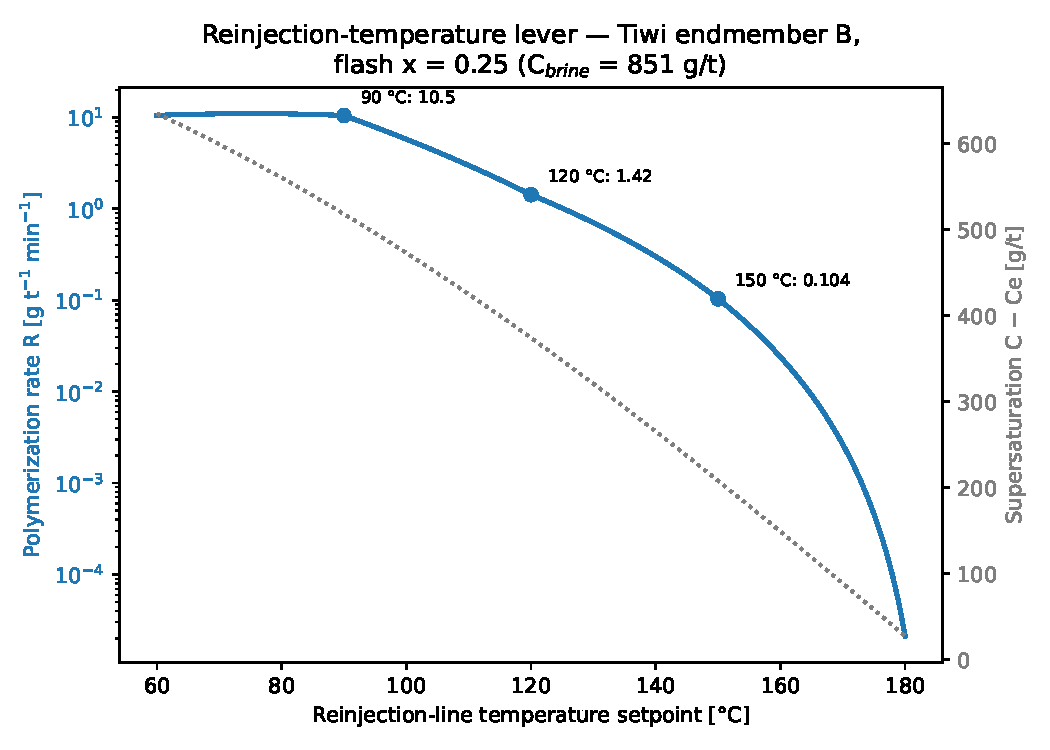
\includegraphics[width=.72\linewidth]{Figure_1}
\caption{The reinjection-temperature lever. Uninhibited polymerization
rate along the brine line versus temperature set-point for the
archetype brine (Tiwi endmember B, 638~mg/kg reservoir
silica~\citep{sugiaman2004geochemical}; flash fraction $x = 0.25$,
scenario input; solubility from \citet{gunnarsson2000amorphous};
kinetics from the checksum-validated transcription of
\citet{rothbaum1979rohde}). Cooling from 150 to 90~$^{\circ}$C raises
the rate by a factor of 101.}\label{fig:lever}
\end{figure}
\begin{figure}[t]\centering
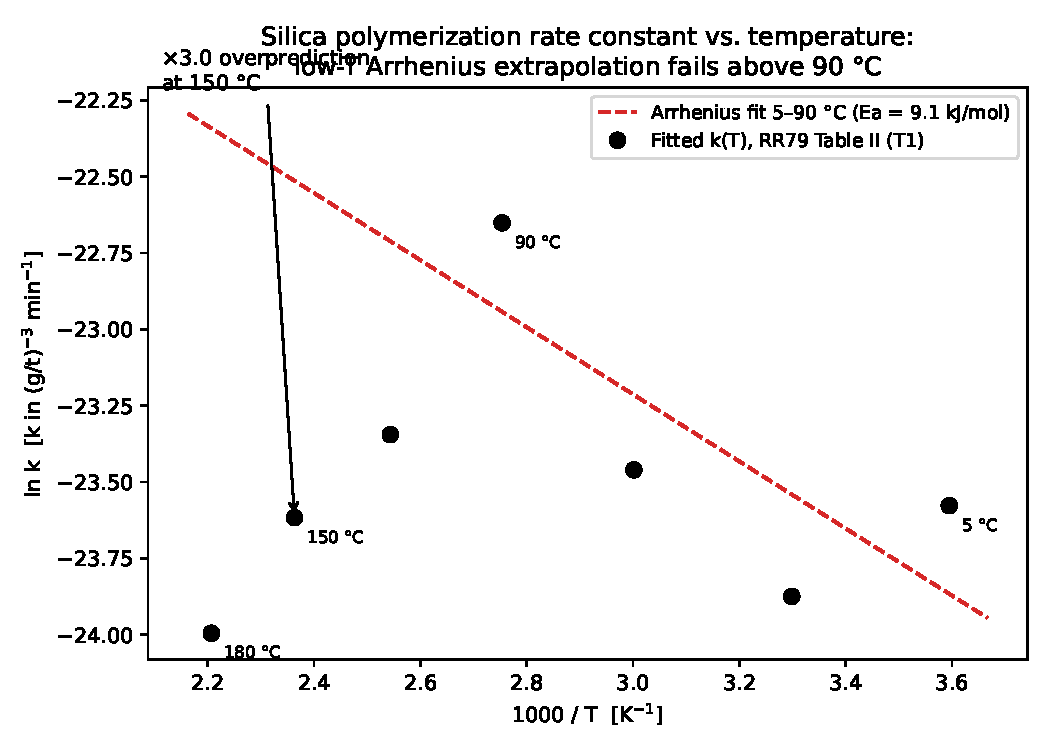
\includegraphics[width=.72\linewidth]{Figure_2}
\caption{Fitted fourth-order rate constants $k(T)$ over
5--180~$^{\circ}$C, regenerated from the primary transcription of
\citet{rothbaum1979rohde}. The dashed Arrhenius fit to the
5--90~$^{\circ}$C nodes ($E_a = 9.1$~kJ/mol) overpredicts $k$ at
150~$^{\circ}$C by a factor of 3.0.}\label{fig:arrhenius}
\end{figure}

\section{Architecture}\label{sec:arch}

\subsection{Synthetic-truth plant}\label{sec:plant}

Performance claims for an estimator or a controller mean little unless
the truth they are tested against differs from the model in ways the
designer did not choose to be easy. We therefore construct a synthetic
plant whose physics is a structurally perturbed instance of the
Section~\ref{sec:benchmark} core, with every deviation parameterized
and documented. The true polymerization rate is
\begin{equation}\label{eq:truth}
r_{\mathrm{true}} \;=\; f_u(u)\, e^{B(T)}\, k(T)\, s^{\,n},
\qquad s = C - C_e(T)\,\beta_e ,
\end{equation}
gated by an induction clock. Here $k(T)$ and $C_e(T)$ are the
literature-fitted core; $B(T)$ is a smooth log-normal bias field drawn
per plant on the seven kinetic isotherm nodes ($\sigma = 0.35$); the
reaction order is drawn as $n \sim \mathcal{N}(4, 0.15)$, clipped to
$[3.6, 4.4]$ in keeping with the ``approximately fourth order'' hedge
of the source data; $\beta_e \sim \mathcal{N}(1, 0.03)$ perturbs
solubility; and $f_u$ is a per-plant perturbed instance of the
non-monotonic dose--response family anchored to field
observations~\citep{gallup2002investigations}, with nominal suppression
of about half near 1~ppm and a mild reversal on overdose. The induction
period is fitted from the primary kinetic dataset itself,
$\log_{10} P = a + b \log_{10} s + cT$ with $b = -4.31$ and
$r^2 = 0.88$, a relation that independently reproduces the source
publication's own graphical correlation. The truth maintains a
supersaturation-exposure clock that the model core deliberately lacks.

Brine chemistry follows a mean-reverting Ornstein--Uhlenbeck
fluctuation of endmember mixture weights around the nominal operating
composition on the Tiwi envelope~\citep{sugiaman2004geochemical}, with
a bounded flash-fraction perturbation. One modeling correction deserves
open mention. An earlier revision used a pure simplex random walk,
which drifts toward the mixture centroid and quietly diluted the brine
from 799 to 579~mg/kg over ten days, relaxing the constraint for every
controller in the study. The mean-reverting form restores stationarity
(a drift of about 1.3\% over ten days), and stationarity is now one of the
repository's automated checks. The measurement layer is deliberately
shift-realistic: silica grab samples every 8~h at 5\% relative noise,
continuous line temperature at $\sigma = 0.3\,^{\circ}$C, and a single
noisy daily observation of the trailing-24-h mean rate (10\% relative
noise, standing in for a coupon or turbidity proxy). A fourteen-day
episode thus provides 42 concentration samples and 14 rate labels
against 2{,}016 hidden truth values. This is the sparse-supervision
regime the architecture is built for. A step-wise simulation interface
reproduces the batch simulator's truth path exactly, verified to
machine precision, so that closed-loop experiments can let the
controller decide each day from what it has actually observed.

\subsection{Credibility-weighted hybrid soft sensor}\label{sec:sensor}

The sensed quantity is the trailing-24-h mean polymerization rate: the
quantity that accumulates scale, and the one the optimization layer
constrains. The sensor is a parallel
hybrid~\citep{thompson1994modeling,vonstosch2014hybrid},
\begin{equation}\label{eq:sensor}
\hat r \;=\; \operatorname{expm1}\!\big(\log(1{+}r_{\mathrm{core}})
\;+\; \lambda\, g_{\theta}(x)\big)_{+},
\end{equation}
in which $r_{\mathrm{core}}$ is the trailing mean of the kinetic core
combined with the nominal literature dose--response, and $g_{\theta}$
is a gradient-boosted residual~\citep{ke2017lightgbm} in
$\log(1{+}\cdot)$ space over causal trailing-window aggregates of
observables only. A code-level guard raises an error if any truth-side
variable reaches the feature set. Training is per plant, on that
plant's own sparse daily labels, under strict temporal splits, which is
the standard soft-sensor protocol~\citep{kadlec2009data}.

The protocol is itself a result. Our first evaluation asked the
residual to generalize zero-shot to unseen truth realizations, and the
hybrid lost to both a pure-physics and a pure-data baseline. The
diagnosis is structural rather than statistical. Per-plant mismatch
draws are unpredictable before any data from that plant exists, so a
zero-shot split tests a claim no soft sensor makes; a soft sensor is
trained on its plant's history and predicts forward in time, where the
plant's own bias is identifiable. We report this negative result
because it motivates the two protective mechanisms that follow. The
residual weight $\lambda$ in Eq.~\eqref{eq:sensor} is set by
leave-one-out (LOO) credibility on the training labels,
\begin{equation}\label{eq:lambda}
\lambda^{\ast} = \operatorname{clip}_{[0,1]}
\frac{\langle e, \tilde r\rangle}{\langle \tilde r, \tilde r\rangle},
\qquad \lambda = 0 \ \text{unless the LOO SSE improves by at least } 15\%,
\end{equation}
where $e$ collects the residual targets and $\tilde r$ their LOO
predictions. The correction is used only to the extent that it
demonstrates out-of-sample signal, and the hybrid falls back gracefully
to its physics prior as labels become few or uninformative. The same
LOO computation yields the residual's prediction-error standard
deviation $\sigma_{\mathrm{LOO}}$, which is exported to the
optimization layer as the sensor's own statement of uncertainty.

\subsection{Robust economic RTO and the feedback schemes compared}\label{sec:rto}

Following the two-layer rationale of steady-state real-time
optimization~\citep{darby2011rto}, the decision variables are the
reinjection temperature set-point and the inhibitor dose, $(T_r, u)$,
refreshed daily. The objective is heat-recovery revenue minus inhibitor
cost, with every economic coefficient declared as a scenario parameter
(peso-denominated; Section~\ref{sec:phcontext}). The scaling constraint
is enforced on every vertex of the brine-chemistry envelope at the
adverse flash bound,
\begin{equation}\label{eq:rto}
\max_{T_r,\,u}\; J(T_r, u)
\quad \text{s.t.} \quad
r_v(T_r, u) \;\le\; r_{\max} \quad \forall v \in \mathcal{V},
\end{equation}
where $r_v = k(T_r)\,(C_v - C_e(T_r))^4 f(u)$ is the kinetic core at
the design-case silica concentration $C_v$ of vertex $v$ and $f$ is the
nominal dose--response. The problem is solved by dense grid
search ($161 \times 81$ points). The choice is deliberate: on a bounded
two-dimensional decision space the grid is global, deterministic and
auditable by any reader, and the vectorized implementation is
consistency-checked against the reference solver at start-up. Solved
once and held, Eq.~\eqref{eq:rto} is the open-loop robust policy.

Once a day the plant returns one noisy label $\ell_t$ of the
trailing-24-h mean rate. We compare three ways of using it. All of them
correct the constraint of Eq.~\eqref{eq:rto} and leave the objective
untouched.

\paragraph{Scalar constraint adaptation} The zeroth-order scheme of
\citet{chachuat2008constraint} filters the constraint bias,
\begin{equation}\label{eq:ca}
\varepsilon_t = (1-\alpha)\,\varepsilon_{t-1}
 + \alpha\,\big(\ell_t - r_a(T_{r,t}, u_t)\big), \qquad
r_v + \varepsilon_t \le r_{\max},
\end{equation}
with $\alpha = 0.5$. A log-space variant filters
$\ln \ell_t - \ln r_a$ and scales the constraint by $e^{\theta_t}$. The
gradient modifiers of full modifier
adaptation~\citep{marchetti2009modifier,marchetti2010dual} are not
attempted, since one noisy label per day does not support estimating
plant gradients. The model $r_a$ against which the innovation is formed
is the \emph{anchor}, and the comparison of Section~\ref{sec:anchoring}
turns on it. With the \emph{design-case anchor}, $r_a = r_B$: the
kinetic core at the composition the optimizer is already solved
against, namely the envelope vertex nearest the operating brine, at the
adverse flash bound. With the \emph{measured anchor},
$r_a = k(T_r)\,(C_m - C_e(T_r))^4 f(u)$, the core at the most recent
silica grab sample $C_m$.

\paragraph{Gaussian-process residual} The constraint model becomes
$\log(1+\hat r_v) = \log(1+r_v) + \mu(x)$, where $\mu$ is the posterior
mean of a Gaussian process trained on the residual targets
$\log(1+\ell_t) - \log(1+r_a)$ at the measured anchor, with inputs
$x = (T_r, u, C_m - C_e)$, a constant mean and a squared-exponential
kernel with one length scale per input plus noise. Hyperparameters are
chosen by exact marginal likelihood over a small fixed grid, so the fit
involves no optimizer and is deterministic. This arm takes from
modifier adaptation with Gaussian
processes~\citep{ferreira2018gpma,delriochanona2021tale} the idea of a
learned mismatch model that reports its own uncertainty. It does not
implement those methods' cost modifiers, acquisition functions or trust
regions, and the results below test the regressor, not those
algorithms.

\paragraph{Hybrid sensor} The trained sensor of
Section~\ref{sec:sensor} is used as the constraint model,
$\log(1+\hat r_v) = \log(1+r_v) + \lambda\, g_\theta(x)$, queried at
steady state across the decision grid. Its residual target and anchor
are those of the Gaussian-process arm. The two differ in the regressor
and in their inputs: the hybrid receives the sensor's full set of
trailing-window features, the Gaussian process the three listed above.

\paragraph{Uncertainty back-off} Each family is backed off by a gain
$\kappa$ times its own uncertainty estimate,
\begin{equation}\label{eq:backoff}
r_v + \varepsilon_t + \kappa\,\sigma_u \le r_{\max}
\quad\text{(scalar)}, \qquad
\log(1+\hat r_v) + \kappa\,\sigma \le \log(1+r_{\max})
\quad\text{(learned)},
\end{equation}
where $\sigma_u$ is the standard deviation of the scalar scheme's
one-step prediction error over the trailing 14 days, and $\sigma$ is
the Gaussian-process predictive standard deviation or the hybrid's
$\sigma_{\mathrm{LOO}}$. We sweep $\kappa \in \{0, 0.5, 1, 2\}$. The
three uncertainty estimates live on different scales, so equal $\kappa$
does not mean equal conservatism across families; the families are
compared as frontier curves over the sweep, not gain by gain.

The learned models are refitted weekly once seven labels exist. Until
then they run the measured-anchored scalar modifier restricted to
tightening ($\varepsilon \ge 0$), so that feedback cannot relax the
constraint before a model has earned credibility.

\section{In-silico results}\label{sec:results}

\subsection{Estimation under sparse labels}\label{sec:table1}

The estimation experiment simulates \NUM{T1plants} independent truth
realizations for 90 days each. Sensors were trained on the first 60 days of labels and
evaluated on the final 30, following the per-plant temporal protocol.
Table~\ref{tab:ablation} summarizes the ablation triple.
\begin{table}[t]\centering
\caption{Estimation ablation on unseen test windows: RMSE in
$\log(1{+}\cdot)$ rate space (mean $\pm$ sd over \NUM{T1plants} plants)
and the fraction of estimates within a factor of two of the hidden
truth. Generated from \texttt{results/table1\_summary.csv}.}
\label{tab:ablation}
\begin{tabular}{lccc}
\toprule
Arm & RMSE$_{\log 1p}$ & vs.\ physics & within $\times 2$ \\
\midrule
% GENERATED by manuscript/make_numbers.py — do not edit
Physics core & $0.346 \pm 0.181$ & --- & 41\% \\
Pure ML & $0.258 \pm 0.069$ & $-25\%$ & 64\% \\
Hybrid & $0.170 \pm 0.037$ & $-51\%$ & 84\% \\

\bottomrule
\end{tabular}
\end{table}
The hybrid reduces error by \NUM{T1redPh}\% against its own physics
prior and by \NUM{T1redMl}\% against the pure-data baseline, and it
places \NUM{T1Hywf}\% of its estimates within a factor of two of the
hidden truth, against \NUM{T1Phwf}\% and \NUM{T1Mlwf}\%. The
label-scarcity sweep in Fig.~\ref{fig:scarcity} sharpens the point.
With \NUM{ScDayMin} days of labels the hybrid (\NUM{ScHyMin}) already
outperforms both the physics core given any amount of data (at best
\NUM{ScPhBest}) and the pure-data arm given all \NUM{ScDayMax} days
(\NUM{ScMlMax}). The transfer experiment bounds the claim: a residual
carried to a foreign plant along with its donor credibility does active
harm (\NUM{TrHy} against the physics prior's \NUM{TrPh}, mean over
\NUM{TrPlants} unseen plants). This is why $\lambda$ must be earned
from the target plant's own labels. At zero labels $\lambda = 0$ and
the hybrid simply is its prior.

\begin{figure}[t]\centering
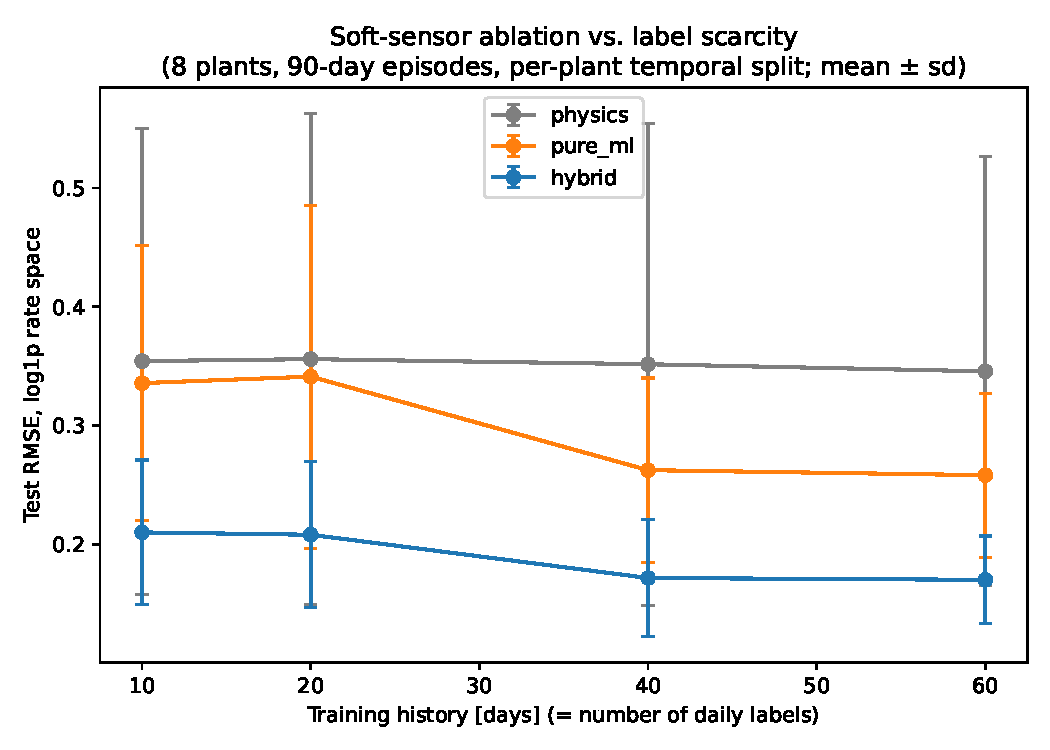
\includegraphics[width=.7\linewidth]{Figure_3}
\caption{Test RMSE versus training-history length, equal to the number
of daily labels; mean $\pm$ sd over \NUM{T1plants} plants. Generated
from \texttt{results/scarcity\_sweep.csv}.}\label{fig:scarcity}
\end{figure}

\subsection{Closed-loop design}\label{sec:stress}

The feedback schemes of Section~\ref{sec:rto} are run in closed loop on
\NUM{CLplantsB} plants for \NUM{CLdays} days each, in two regimes. The
\emph{benign} regime uses the random per-plant mismatch of
Section~\ref{sec:plant}. The \emph{stress} regime is a deterministic
single-factor perturbation: the plant's true rate is six times the
model's, with all random draws zeroed. Its magnitude is a measurement,
not a choice, being the median gap between the fitted core and
independent modern kinetics found in Section~\ref{sec:validation}.

A violation day is a day whose realized trailing-24-h mean rate exceeds
$r_{\max}$. Violations are counted on the realized plant, not on the
worst-case vertex of the envelope, from day 2 (total) and from day 9
(post-warm-up). Uplift is gross power relative to fixed empirical
practice at 150~$^{\circ}$C with 1~ppm continuous dosing, the pattern
of documented field programs~\citep{baltazar2014grc}. Every arm sees
the same brine and mismatch realization on a given plant, so arms are
compared by paired differences over plants, with seeded
percentile-bootstrap 95\% intervals (4{,}000 resamples, plants as the
resampling unit).

Two kinds of evidence are kept apart. Six of the twenty plants per
regime, with the hybrid arm at $\kappa \in \{0, 1\}$ against the
open-loop policy, formed a protocol whose pass criteria were fixed
before its runs. Those verdicts are reported as registered at the end
of Section~\ref{sec:models}. Everything else in
Sections~\ref{sec:anchoring} and~\ref{sec:models}, that is the
anchoring ablation, the scalar and Gaussian-process families, the gain
sweep and the fourteen further plants, was added afterwards with
earlier results in view. It is post hoc and should be read as such.
Table~\ref{tab:closedloop} and Fig.~\ref{fig:frontier} give the full
results.

\begin{table}[!tbp]\centering\footnotesize
\setlength{\tabcolsep}{3.2pt}\renewcommand{\arraystretch}{0.78}
\caption{Closed-loop results, mean over \NUM{CLplantsB} plants
$\times$ \NUM{CLdays} d per regime. Uplift is gross power over fixed
practice (mean $\pm$ sd over plants, \%). Violation days are means per
episode with the worst plant in parentheses; ``post-w.'' counts days
after the 8-day warm-up. Generated from
\texttt{results/table2\_summary.csv} and
\texttt{results/table2b\_summary.csv}.}
\label{tab:closedloop}
\begin{tabular}{lccccc}
\toprule
 & \multicolumn{2}{c}{Benign regime} & \multicolumn{3}{c}{Stress regime
 ($\times 6$)} \\
\cmidrule(lr){2-3}\cmidrule(lr){4-6}
Arm & Uplift & Viol.\ days & Uplift & Viol.\ days & Post-w. \\
\midrule
% GENERATED by manuscript/make_numbers.py — do not edit
Fixed practice & --- & 0.00 (0) & --- & 0.00 (0) & 0.00 \\
Robust RTO, no feedback & $+41.7 \pm 0.0$ & 0.45 (7) & $+41.7 \pm 0.0$ & 20.65 (28) & 17.50 \\
\addlinespace
\multicolumn{6}{l}{\emph{Anchoring ablation (scalar constraint adaptation, by anchor)}} \\
\quad additive, design case & $+81.5 \pm 20.7$ & 5.60 (17) & $+37.3 \pm 2.5$ & 15.80 (18) & 13.25 \\
\quad log-space, design case & $+100.3 \pm 33.5$ & 17.80 (21) & $+41.3 \pm 3.2$ & 19.20 (26) & 16.35 \\
\quad log-space, measured & $+3.4 \pm 52.2$ & 0.35 (2) & $-46.7 \pm 15.7$ & 0.25 (1) & 0.15 \\
\quad additive, measured ($\kappa{=}0$) & $+40.6 \pm 7.1$ & 0.00 (0) & $+21.1 \pm 1.5$ & 1.60 (6) & 1.25 \\
\addlinespace
\multicolumn{6}{l}{\emph{Scalar modifier, measured anchor, back-off gain $\kappa$}} \\
\quad $\kappa = 0$ & $+40.6 \pm 7.1$ & 0.00 (0) & $+21.1 \pm 1.5$ & 1.60 (6) & 1.25 \\
\quad $\kappa = 0.5$ & $+34.8 \pm 6.1$ & 0.00 (0) & $+15.9 \pm 2.0$ & 0.65 (2) & 0.45 \\
\quad $\kappa = 1$ & $+29.3 \pm 5.6$ & 0.00 (0) & $+10.6 \pm 2.6$ & 0.40 (1) & 0.20 \\
\quad $\kappa = 2$ & $+18.6 \pm 6.6$ & 0.00 (0) & $-1.1 \pm 4.5$ & 0.25 (1) & 0.05 \\
\addlinespace
\multicolumn{6}{l}{\emph{GP residual, measured anchor, back-off gain $\kappa$}} \\
\quad $\kappa = 0$ & $+41.1 \pm 8.5$ & 0.10 (2) & $+19.7 \pm 3.1$ & 1.90 (5) & 1.45 \\
\quad $\kappa = 0.5$ & $+37.0 \pm 9.0$ & 0.05 (1) & $+14.2 \pm 3.1$ & 0.85 (3) & 0.50 \\
\quad $\kappa = 1$ & $+31.3 \pm 10.7$ & 0.00 (0) & $+7.1 \pm 4.6$ & 0.60 (2) & 0.25 \\
\quad $\kappa = 2$ & $+14.8 \pm 11.3$ & 0.00 (0) & $-13.1 \pm 6.9$ & 0.95 (6) & 0.60 \\
\addlinespace
\multicolumn{6}{l}{\emph{Hybrid sensor, measured anchor, back-off gain $\kappa$}} \\
\quad $\kappa = 0$ & $+42.0 \pm 6.8$ & 0.15 (2) & $+23.6 \pm 2.5$ & 3.60 (9) & 3.15 \\
\quad $\kappa = 0.5$ & $+38.0 \pm 7.2$ & 0.00 (0) & $+17.9 \pm 2.7$ & 1.40 (3) & 1.05 \\
\quad $\kappa = 1$ & $+34.1 \pm 7.6$ & 0.05 (1) & $+13.3 \pm 2.1$ & 0.75 (2) & 0.40 \\
\quad $\kappa = 2$ & $+25.7 \pm 9.2$ & 0.00 (0) & $+2.7 \pm 5.6$ & 0.40 (1) & 0.05 \\

\bottomrule
\end{tabular}
\end{table}

\begin{figure}[!tbp]\centering
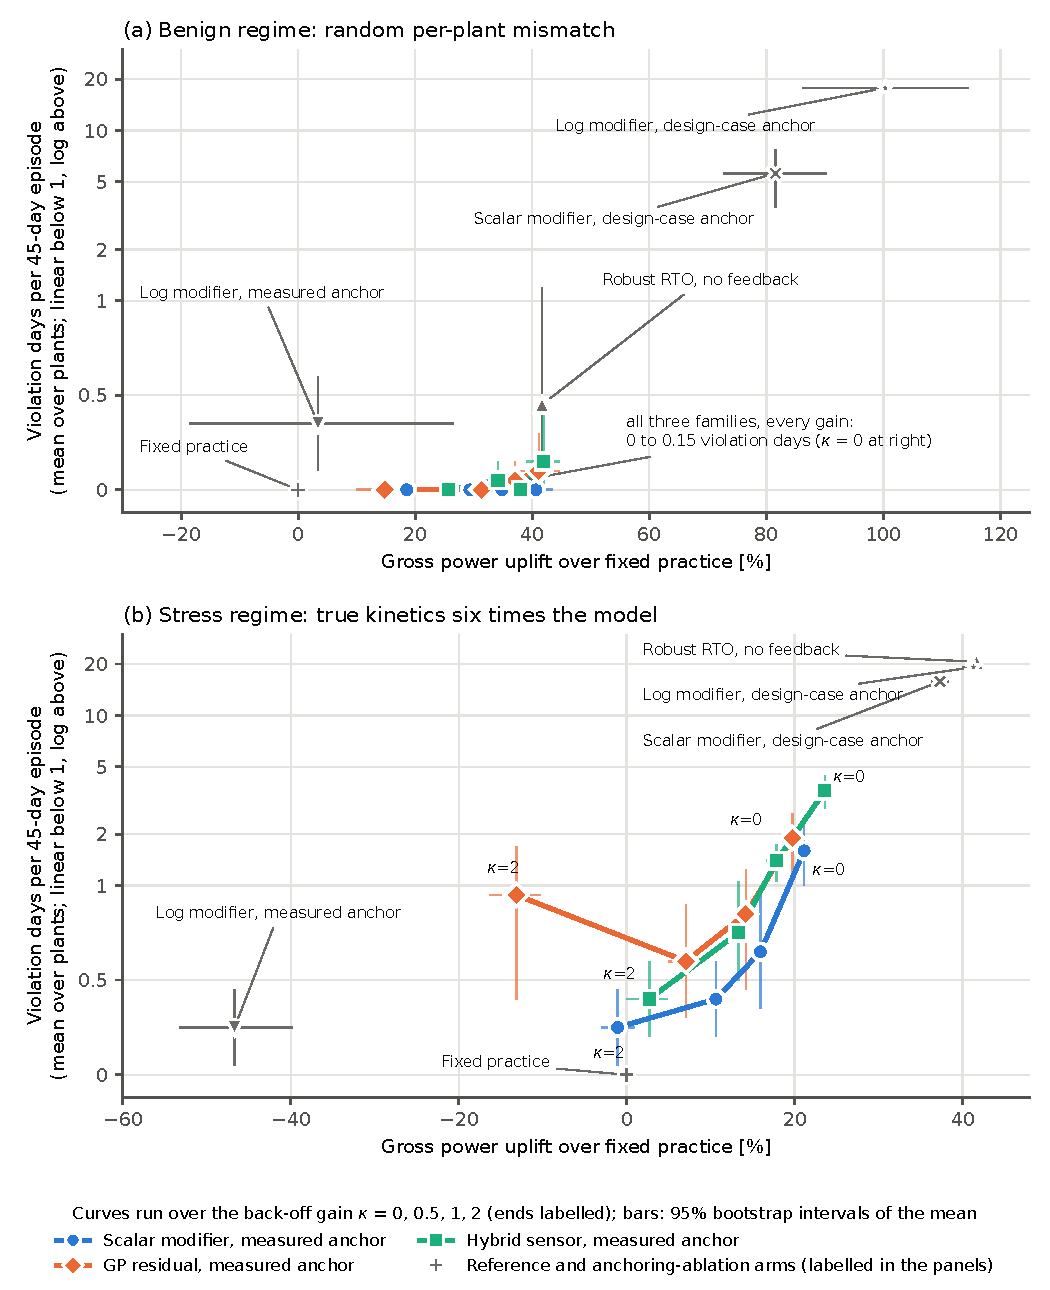
\includegraphics[width=\linewidth]{Figure_4}
\caption{Safety--harvest view of Table~\ref{tab:closedloop}. Each
measured-anchored family is a curve over the back-off gain
$\kappa = 0, 0.5, 1, 2$, with $\kappa = 0$ at the high-uplift end;
reference and anchoring-ablation arms are single labelled markers. Bars
are 95\% bootstrap intervals of the mean over plants. The vertical axis
is linear below one violation day and logarithmic above. Generated from
\texttt{results/closed\_loop\_frontier.csv}.}\label{fig:frontier}
\end{figure}

\subsection{The anchor decides safety}\label{sec:anchoring}

Consider the anchoring block of Table~\ref{tab:closedloop}. With the
design-case anchor the additive modifier averages \CL{B}{CAnom}{v}
violation days per episode in the benign regime (\CL{B}{CAnom}{m} on
the worst plant) and \CL{S}{CAnom}{v} under stress, against
\CL{S}{Open}{v} with no feedback at all. With the measured
anchor the same modifier, at the same gain, averages \CL{B}{CAk0}{v}
and \CL{S}{CAk0}{v}. The paired reductions are \CT{anchorB}{v}{abs}
days (95\% interval \CT{anchorB}{v}{lop} to \CT{anchorB}{v}{hip}) and
\CT{anchorS}{v}{abs} days (\CT{anchorS}{v}{lop} to
\CT{anchorS}{v}{hip}). The log-space modifier behaves the same way
under stress, at \CL{S}{LGnom}{v} against \CL{S}{LGmeas}{v} violation
days.

A diagnostic isolates the mechanism. Hold the operating point fixed at
the open-loop optimum on the \NUM{AnPlants} stress plants, so that the
model error a feedback scheme ought to see is a constant factor of six,
and form each day the ratio of the label to the anchor model. The
design-case composition is more concentrated than the brine the plant
actually sees, so through the fourth-power rate law the design-case
model over-predicts the realized-brine model by a median factor of
\NUM{AnMarginmed}. That factor is the robust optimizer's safety margin.
An innovation formed at the design case contains the product of the
margin and the model error and cannot separate them. Under the sixfold
stress the two nearly cancel: the ratio of label to design-case model
has a median of \NUM{AnDesmed} (5th to 95th percentile \NUM{AnDeslo} to
\NUM{AnDeshi}), the modifier sees almost nothing to correct, and the
plant is left at an operating point where the realized rate exceeds
the limit on \NUM{AnShare}\% of days. In the benign regime, where there
is no systematic kinetic error, the same innovation reads the margin as
conservatism, relaxes the constraint, harvests an uplift of
\CL{B}{CAnom}{u}\% and violates. Formed at the measured silica, the
ratio has a median of \NUM{AnMeasmed}, close to the kinetic error it
should see.

That the margin and the stress are of nearly equal size in this
benchmark is a coincidence. The confounding is not. A scheme that
solves against a worst-case envelope and adapts on plant feedback must
form its innovation at the realized disturbance, or it will mistake its
own robustness margin for mismatch, in whichever direction the two
happen to combine.

The diagnostic also explains a secondary result. The measured-anchored
ratio is heavy-tailed (95th percentile \NUM{AnMeashi}), because on some
days the measured supersaturation is small and the model rate nearly
vanishes. The additive modifier is insensitive to that tail, since a
small model rate produces a small absolute innovation. The log-space
modifier is not: at the measured anchor it is safe but so conservative
that under stress it runs hotter than fixed practice
(\CL{S}{LGmeas}{u}\% uplift).

\subsection{Correction model and back-off gain}\label{sec:models}

\paragraph{Benign regime} Once anchored to the measurement, all three
families are essentially violation-free. At $\kappa = 0$ the scalar
modifier has no violation day on any of the \NUM{CLplantsB} plants, the
Gaussian-process residual averages \CL{B}{GPk0}{v} and the hybrid
\CL{B}{HYk0}{v}, at uplifts of \CL{B}{CAk0}{u}\%, \CL{B}{GPk0}{u}\% and
\CL{B}{HYk0}{u}\%. These uplifts are those of the open-loop robust
policy (\CL{B}{Open}{u}\%), which, however, leaks: \CL{B}{Open}{v}
violation days on average and \CL{B}{Open}{m} on its worst plant,
because an envelope over brine chemistry does not certify against
kinetic draws. In this regime feedback buys safety rather than harvest,
and back-off costs harvest while buying nothing. Inhibitor intensity
falls from \CL{B}{Fixed}{i}~PHP/MWh under fixed practice to
\CL{B}{CAk0}{i}~PHP/MWh.

\paragraph{Stress regime} Under the sixfold kinetic error the
open-loop policy violates on \CL{S}{Open}{v} of 44 counted days, and
the three measured-anchored families separate into the frontier curves
of Fig.~\ref{fig:frontier}(b). Without back-off the scalar modifier
holds an uplift of \CL{S}{CAk0}{u}\% at \CL{S}{CAk0}{v} violation days.
The hybrid harvests slightly more (\CL{S}{HYk0}{u}\%) and violates more
(\CL{S}{HYk0}{v} days; paired difference \CT{HYk0S}{v}{d}, interval
\CT{HYk0S}{v}{lop} to \CT{HYk0S}{v}{hip}). The Gaussian-process
residual harvests slightly less (\CL{S}{GPk0}{u}\%) at a violation
count indistinguishable from the scalar's (difference
\CT{GPk0S}{v}{d}, interval \CT{GPk0S}{v}{lop} to \CT{GPk0S}{v}{hip}).

Back-off moves every family along its curve at a similar price. Going
from $\kappa = 0$ to $\kappa = 1$ costs the scalar modifier
\CT{boCA}{u}{abs} points of uplift and removes \CT{boCA}{v}{abs}
violation days; for the hybrid the figures are \CT{boHY}{u}{abs} points
and \CT{boHY}{v}{abs} days, and for the Gaussian process
\CT{boGP}{u}{abs} points and \CT{boGP}{v}{abs} days. At $\kappa = 2$
the scalar and hybrid families are down to \CL{S}{CAk2}{w} and
\CL{S}{HYk2}{w} post-warm-up violation days respectively, with almost
no harvest left (\CL{S}{CAk2}{u}\% and \CL{S}{HYk2}{u}\%). Under a sixfold kinetic
error there is little harvest that is safe to take.

Read as frontiers, the families overlap, and no learned model
dominates the scalar modifier. At equal gain the hybrid sits a few
points of uplift to the right of the scalar curve and somewhat above it
(at $\kappa = 1$: \CT{HYk1S}{u}{d} points, \CT{HYk1S}{v}{d} violation
days), which is a different point on a similar curve, not a better
curve. The Gaussian-process family lies weakly inside the scalar one,
with less uplift at every gain and, at $\kappa = 2$, more violations as
well (\CT{GPk2S}{u}{d} points, \CT{GPk2S}{v}{d} days). A plausible
reason is that a wide posterior away from the visited operating points
pushes the optimizer into regions the model has not seen, which is the
failure that trust regions address in the Gaussian-process
literature~\citep{delriochanona2021tale}.

We offer two explanations, neither of which the experiments isolate.
The first is that a plant regulated near one operating point needs a
correction that is local and current, and a scalar updated every day
supplies exactly that, whereas the learned models are refitted weekly.
The second concerns the hybrid specifically. Credibility shrinkage
pulls the correction toward the kinetic prior. That protects estimation
accuracy, but when the prior under-predicts sixfold it is the unsafe
direction, and the hybrid without back-off duly has the most violations
of the three families.

\paragraph{Registered verdicts} On the six plants of the registered
protocol, the open-loop policy violates chronically (\NUM{PreOpenv}
days), as expected. The hybrid without back-off averages
\NUM{PreHYk0w} post-warm-up violation days; the target first
registered for that arm was zero, and it was missed. The hybrid with
$\kappa = 1$ averages \NUM{PreHYk1w} days against a registered
criterion of at most 0.5, and it is safer than the arm without
back-off, as registered. These figures use the corrected,
measured-anchored warm-up. With the original design-case warm-up the
two arms gave 2.17 and 0.50 days, and the verdicts were the same; those
runs remain reproducible from the repository.

\subsection{Global sensitivity and economic ranges}\label{sec:sobol}

A Sobol study ($N = \NUM{SobN}$, seeded, \NUM{SobEvals} evaluations)
spans the declared uncertainty set: a kinetic band equal to the
measured sixfold gap, a solubility band equal to the measured endpoint
spread $[0.90, 1.37]$, and declared scenario bands for flash,
dose--response, $r_{\max}$ and economics (Fig.~\ref{fig:sobol}).
Kinetic model-family uncertainty dominates the economics of the
open-loop optimum, with total-order indices of \NUM{SobSTMw},
\NUM{SobSTT} and \NUM{SobSTNet} on gross power, optimal temperature and
net objective. The optimal dose is governed instead by dose--response
knowledge ($S_T = \NUM{SobSTDose}$), which identifies inhibitor
characterization as the second identification target. Feasibility
holds at \NUM{SobFeas}\% across the set, so the declared uncertainty
never strands the optimizer, and the gross-power optimum spans
\NUM{Sobmwq05}/\NUM{Sobmwq50}/\NUM{Sobmwq95}~MW
($q_{05}/q_{50}/q_{95}$). Finally, re-valuing the closed-loop
trajectories over the economics envelope attaches ranges to every peso
figure. The enabling assumption is verified, not assumed: the optimum
moves zero grid steps across all eight envelope corners, with inhibitor
cost below 15\% of revenue everywhere, so uplift percentages and
violation counts are untouched. The safety conclusions of
Table~\ref{tab:closedloop} do not depend on economic assumptions.

\begin{figure}[t]\centering
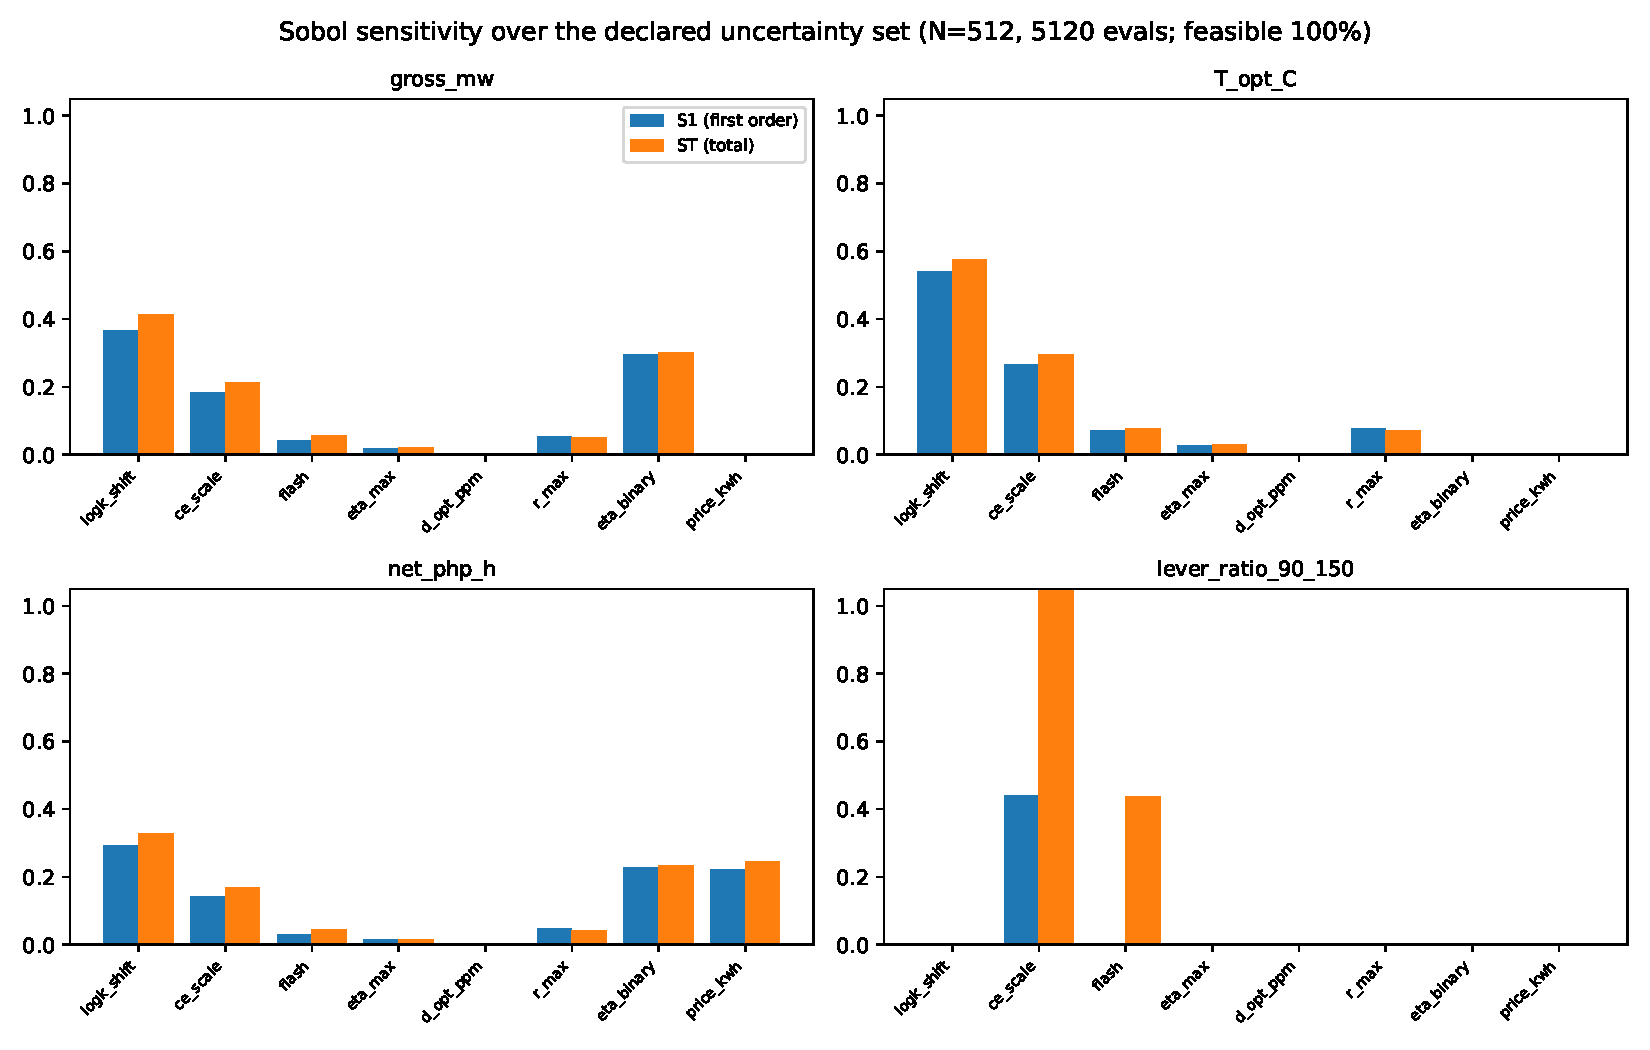
\includegraphics[width=.95\linewidth]{Figure_5}
\caption{First- and total-order Sobol indices over the declared
uncertainty set. Generated from
\texttt{results/sensitivity\_sobol.csv}.}
\label{fig:sobol}
\end{figure}

\section{Out-of-sample validation on independent data}\label{sec:validation}

Every physics component of the architecture, and the sensing pattern
itself, is confronted with an experimental dataset it was never fitted
to: the supplementary data of \citet{scott2024silica}, read with the
parameterization corrections of \citet{scott2024corrigendum}. The
corpus comprises 61 monomeric-silica decay experiments and 1{,}275
points spanning 23--80~$^{\circ}$C, pH 2.1--10.0 and ionic strength
0.01--0.53~mol/kg. Because the source is machine-readable, manual
transcription protocols give way to automated parser integrity checks:
unit-header pinning, monotonicity, separation of replicate runs listed
under duplicated identifiers, and flagging of one colloid-regime
outlier that falls outside the dissolved-monomer scope.

\subsection{Kinetics: what a 1979 law does and does not predict}

Two properties of the fitted core are tested separately, because they
fail differently. Consider first the functional form. Linearizing the
integrated $n$-th-order decay law and sweeping $n \in \{2,\dots,6\}$
per experiment shows that single-curve monomer decay in the modern data
is cleanly second order in supersaturation: median $R^2 = 0.992$ at
$n = 2$, degrading monotonically as the assumed order rises, with
best-fit order 2 in all eleven qualifying near-neutral experiments
(Fig.~\ref{fig:kinval}). This does not contradict the source of the
core. The classical ``fourth order'' is a correlation of maximum rate
against initial supersaturation across separate batches, a peak-rate
law, whereas the integrated decay of a single curve follows
Rimstidt--Barnes-type second-order
kinetics~\citep{rimstidt1980kinetics}. The two describe different
observables, and we report both rather than forcing either onto data
that says otherwise. Now the rate level. The observed second-order
constants follow an Arrhenius trend with $E_a \approx 22$~kJ/mol, and
the effective decay constant implied by the fitted core differs from
observation by a factor of about six at the median. That number does
double duty in this paper. It calibrates the adverse stress of
Section~\ref{sec:stress}, and it is the measured size of the gap that
any feedback scheme on this process has to absorb: no single
transcribed rate law reproduces independent modern data.

\begin{figure}[t]\centering
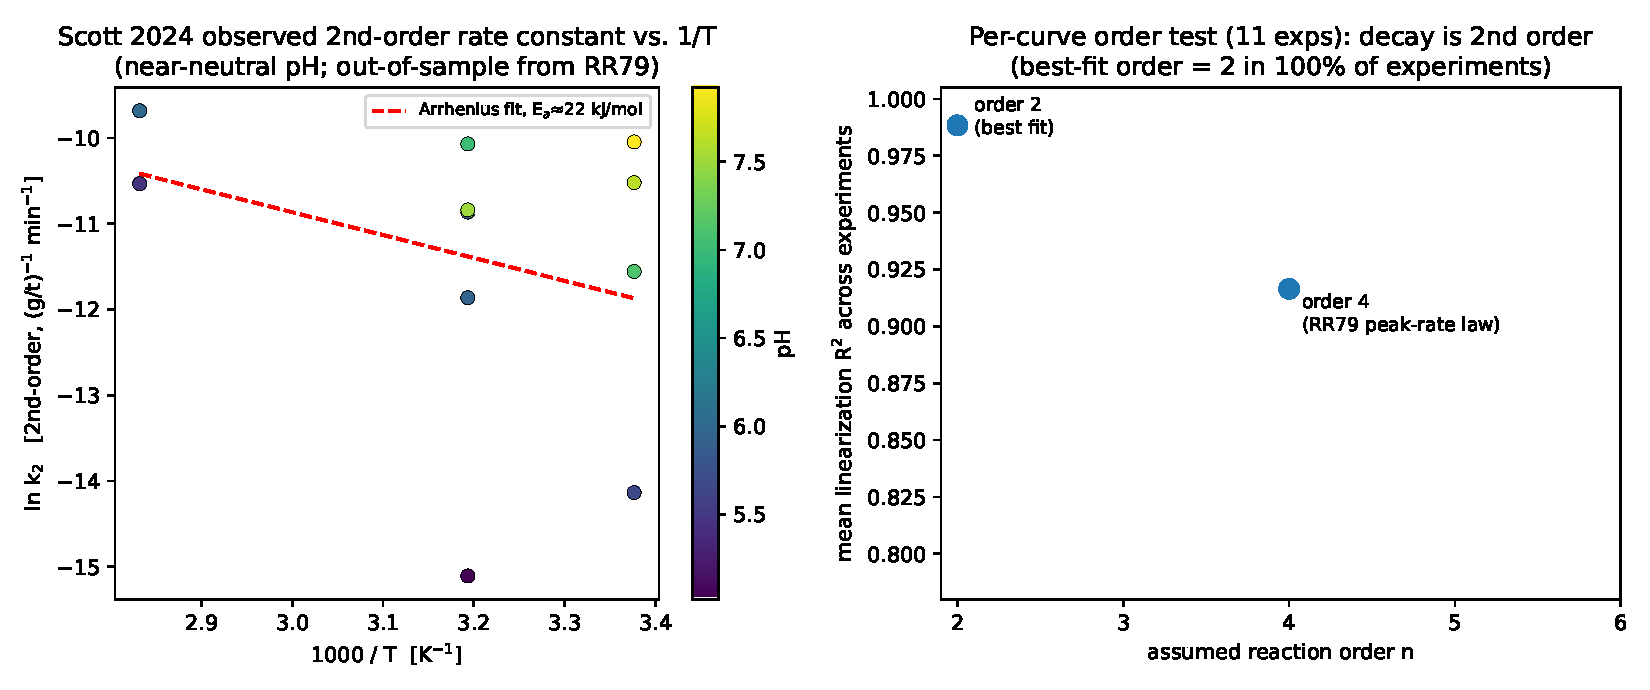
\includegraphics[width=.95\linewidth]{Figure_6}
\caption{Out-of-sample kinetic validation against
\citet{scott2024silica}. Left: observed second-order rate constants
versus inverse temperature for the near-neutral experiments, with the
Arrhenius trend. Right: mean linearization $R^2$ versus assumed
reaction order; single-curve decay is second order, while the
fourth-order form is a peak-rate law. Source:
\texttt{results/kinetics\_validation.csv}.}
\label{fig:kinval}
\end{figure}

\subsection{Solubility: mutual validation across 24 years}

The plateau of a near-complete decay experiment is an independent
measurement of amorphous-silica solubility. Sixteen near-neutral
experiments that consumed at least 70\% of their initial
supersaturation plateau at 0.90--1.37 times the
\citet{gunnarsson2000amorphous} correlation, with a median of 1.05. The
2000 correlation and the 2024 endpoints therefore validate each other
in both directions, and the measured band $[0.90, 1.37]$ becomes the
solubility axis of the sensitivity study in Section~\ref{sec:sobol}.

\subsection{The sensing pattern on real curves: identifiability
precedes correction}\label{sec:sensorval}

Finally, the field sensing pattern is replayed on laboratory truth.
Each qualifying experiment is treated as a plant, interval-average
observed rates as the hidden truth, the fitted core as the prior, and
only the first $K$ intervals as labels. Three arms with honestly
counted parameters are compared: the core alone; a one-parameter scalar
hybrid, a fitted log-level offset that is deployable from a single
label, where a data-only fit cannot operate at all; and a two-parameter
affine hybrid whose slope in $\ln s$ is, by construction, an order
correction. Second-order truth against a fourth-order core predicts
$b \approx -2$.

The raw affine arm is retained as a cautionary ablation. Early labels
span almost no state (a label $\ln s$ spread of 0.047 against a test
span of 2.61), so unregularized slopes explode, with $b$ ranging from
$-230$ to $+769$, and the arm performs far worse than no correction at
all. Applying the same credibility mechanism as the field sensor, a
leave-one-out selection between the scalar and a clipped affine, the
correction collapses to the safe scalar whenever the labels have not
earned the slope ($K \le 3$). At $K = 5$ it engages in 9 of the 19
experiments long enough to be scored with median $b = -2.50$, independently re-measuring the
order-2 finding, and wins outright with a median RMSE of 2.59 against
3.04 for the core (Fig.~\ref{fig:sensorval}). The principle this
crystallizes, identifiability precedes correction, also explains the
in-silico results of Section~\ref{sec:results}. A plant regulated near
an operating point presents a level-dominated, label-covered
correction problem. That is where a hybrid residual estimates well,
and it is also why, in closed loop, a scalar level correction proved
sufficient. Wide-range extrapolation demands state-spanning labels,
and a credible architecture must know which regime it is in.

\begin{figure}[t]\centering
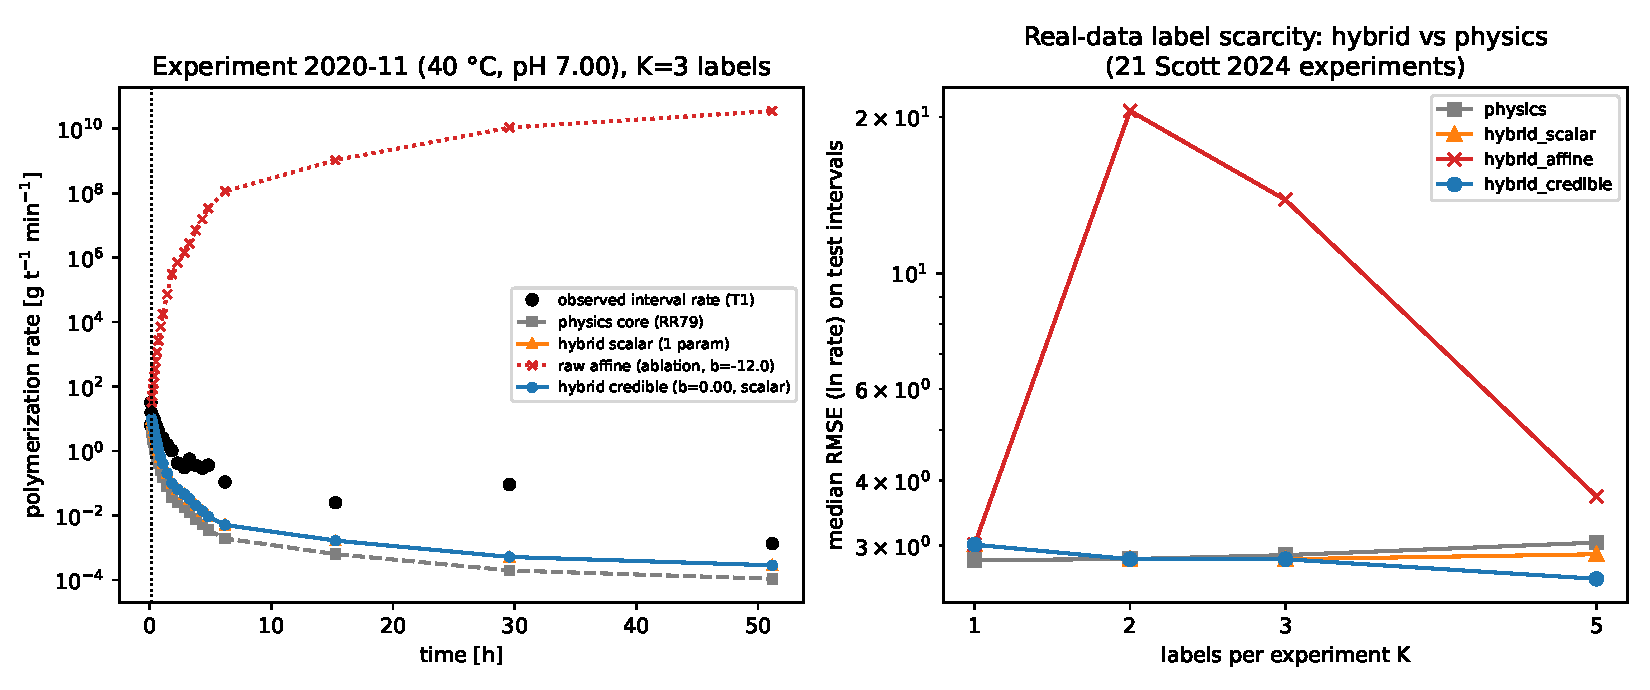
\includegraphics[width=.95\linewidth]{Figure_7}
\caption{The sensing pattern on real decay curves. Left: a
representative experiment, showing the observed interval rates, the
diverging physics core, the raw-affine explosion, and the credible
hybrid. Right: median test RMSE versus labels per experiment $K$ for
all arms, on a log scale. Source:
\texttt{results/sensor\_validation\_scott.csv}.}
\label{fig:sensorval}
\end{figure}

\section{Discussion and limitations}\label{sec:discussion}

\paragraph{What the comparison shows, and what it does not} Two
results are robust across both regimes and all twenty plants: forming
the innovation at the design case fails, and forming it at the
measurement works, for every correction model tried. The ranking among
the measured-anchored families is a weaker statement. It holds for a
plant regulated near one operating point, with one label per day, a
weekly refit of the learned models, and the particular regressors and
uncertainty estimates used here. A plant whose operating point must
move quickly, for example when wells are switched and the brine
composition steps, would favour a correction that is state-dependent
over one that is merely current, and we have not tested that case. The
Gaussian-process arm is a regressor comparison and not an
implementation of Gaussian-process modifier adaptation, whose trust
regions and acquisition functions might well change its curve. Gradient
modifiers were not attempted at all.

\paragraph{Post hoc status of the anchoring result} The anchoring
ablation exists because an earlier version of this study used the
design-case anchor for its scalar baseline and concluded, wrongly, that
the hybrid loop was the only safe policy. The ablation, the
measured-anchored scalar family, the Gaussian-process comparator, the
gain sweep and fourteen of the twenty plants were all added after that
error was found. The effect of the anchor is an order of magnitude in
violation days with intervals far from zero, and it comes with a
mechanism that a separate diagnostic reproduces, so we consider it
secure. The finer comparisons among families were not registered in
advance and would merit replication on an independent benchmark.

\paragraph{How violations are counted} Violations are counted on the
realized plant. Every feedback arm, by tightening or relaxing the
constraint from what the plant returns, trades the worst-case guarantee
of Eq.~\eqref{eq:rto} for performance at the realized brine. Under the
sixfold stress a policy that kept the full envelope guarantee would
have to run hotter than fixed practice, which is what the log-space
modifier at the measured anchor does. The additive corrections are
safe on the realized plant and would under-correct if the brine moved
to the worst-case vertex.

\paragraph{Evaluation posture} The closed-loop results are in silico.
The plant is synthetic, though every physical ingredient, from
solubility and kinetics to the brine envelope and the actuator family,
is grounded in primary literature and, wherever independent data
exists, validated out-of-sample component by component
(Section~\ref{sec:validation}). We regard component-wise real-data
validation combined with a parameterized-mismatch closed loop as the
honest intermediate between simulation-only studies and a field trial.
A field pilot is the natural next step, and it would need only the
sparse instrumentation assumed here.

\paragraph{Constraint units} The scaling constraint is expressed as a
polymerization (monomer-depletion) rate, not as a wall-deposition
thickness rate. The molecular-deposition treatment of
\citet{weres1981kinetics}, transcribed under the same integrity
protocol (its printed checkpoints reproduce, including the 3.0~kcal/mol
effective activation energy; one internal inconsistency in its
Eq.~[4c] is documented and not silently repaired), closes the unit gap.
Along the envelope where the constraint is active,
$r_{\max} = 0.5$~g\,t$^{-1}$\,min$^{-1}$ corresponds to a Weres-implied
molecular-deposition wall growth, a lower bound on total scale growth,
of about 0.3~mm/yr at the optimized operating point and 0.04 to
1.6~mm/yr across 90--175~$^{\circ}$C; the four-fold $r_{\max}$ band of
the sensitivity study spans that calibration.

\paragraph{Scenario fencing and scope} Trade-press figures inform
scenario scale only, a rule enforced mechanically in the repository,
and every peso and megawatt headline carries an envelope range with
decision invariance verified. High-pH brines require silica ionization
corrections that are deferred here; the speciation layer exists in the
repository but is not exercised in the loop.

\paragraph{What generalizes} The anchoring result is not specific to
silica. Whenever an optimizer is solved against a worst-case
disturbance envelope and corrected from plant feedback, the innovation
has to be formed at the realized disturbance, because at the design
case it carries the robustness margin as well as the model error. The
steeper the constraint, the larger the margin in rate terms and the
worse the confusion; here a composition difference of a few percent
becomes a sixfold difference in rate. The same care applies to fouling,
crystallization, corrosion and membrane scaling. The second lesson is
more modest: on this benchmark, a better estimator did not make a
better controller, and the simplest correction that used the right
measurement was as good as any.

\section{Conclusions}\label{sec:conclusions}

We posed geothermal silica scaling as what it is for a process systems
engineer: a hard-constrained economic optimization run against a model
known to be structurally wrong, with the size of the wrongness measured
at a sixfold median gap against independent modern kinetics. Three
results stand. A hybrid soft sensor with a credibility-weighted
residual estimates the scaling rate from sparse daily labels with
\NUM{T1redPh}\% less error than its kinetic core and \NUM{T1redMl}\%
less than a purely data-driven model, and a residual transferred from
another plant does harm, which fixes how such a sensor may be deployed.
In closed loop, what the feedback is anchored to matters more than
which model carries it: a constraint modifier whose innovation is
formed at the robust optimizer's design-case composition confounds
safety margin with model error and averages \CL{S}{CAnom}{v} violation
days per 45-day episode under the sixfold stress, against
\CL{S}{CAk0}{v} for the same modifier anchored to the measured silica.
And once the anchor is right, scalar, Gaussian-process and hybrid
corrections trace overlapping safety--harvest frontiers; the hybrid
sensor's advantage in estimation did not become an advantage in
control, and an uncertainty back-off buys safety from any of them at
roughly ten points of power uplift per unit gain.

The hypothesis this study set out with, that a learned,
uncertainty-aware correction would outperform scalar adaptation, is
therefore not supported on this benchmark, and an earlier version of
the work that seemed to support it did so through a mis-anchored
baseline. The out-of-sample validation is unaffected by that history.
It returned two findings of independent geochemical interest, that
single-curve decay is second order against the classical fourth-order
peak-rate law and that the 2000 solubility correlation and the 2024
endpoints agree at a median of $1.05\times$, together with a design
principle that the closed-loop comparison ended up illustrating from
another side: identifiability precedes correction.

\section*{CRediT authorship contribution statement}
\textbf{Bien Don Busico:} Conceptualization, Methodology, Software,
Validation, Formal analysis, Investigation, Data curation,
Visualization, Writing -- original draft, Writing -- review \& editing.

\section*{Declaration of competing interest}
The author declares that he has no known competing financial interests
or personal relationships that could have appeared to influence the
work reported in this paper.

\section*{Declaration of generative AI and AI-assisted\\ technologies in the manuscript preparation process}
During the preparation of this work the author used Claude (Anthropic)
in order to draft and edit the text of the manuscript and to organize
its structure. After using this tool, the author reviewed and edited
the content as needed and takes full responsibility for the content of
the published article. The use of the same tool in developing the
analysis software is described in \ref{app:repro}.

\section*{Funding}
This research did not receive any specific grant from funding agencies
in the public, commercial, or not-for-profit sectors.

\section*{Data availability}
The code, the transcribed primary data, all result files and the
scripts that regenerate every table and figure are available at\\
\url{https://github.com/beebzy-droid/e1-geothermal-silica-rto}. The
independent validation dataset is the supplementary material of
\citet{scott2024silica} and is obtained from that article; it is not
redistributed.

\section*{Acknowledgments}
The author thanks Dr.~Samuel Scott for directing him to the study's
supplementary dataset, for clarifying the published parameterization
and its corrigendum, and for providing a reference implementation
script used for cross-checking, which is not redistributed with this
work.


\appendix
\section{Data transcription and integrity protocol}\label{app:protocol}
Primary numerical sources enter the repository only through a
transcription protocol: tables are transcribed to CSV against the
publisher's text layer, validated against printed derived quantities
where the source provides them (for the kinetic dataset of
\citet{rothbaum1979rohde}, the printed $R \cdot P^{1.5}$ checksum column
validates 33 of 33 retained rows; one flagged row is excluded), and
tagged with an evidence tier: T1 for peer-reviewed primary sources, T2
for conference or institutional material, and T3 for trade press, which
may motivate scenario scale only and is never fitted, a rule enforced
in code. Machine-readable sources replace manual transcription with
automated parser integrity checks (Section~\ref{sec:validation}).

\section{Reproducibility and software development}\label{app:repro}
A single gate script executes the self-checks of all \NUM{GateModules}
modules (\NUM{GateChecks} checks at the time of writing) and refuses a
green status unless every check passes; the repository convention is
that no commit is made against a red gate. All stochastic components
are seeded, including the Sobol sampler, whose default scrambled
quasi-random sequence is pinned, and the Gaussian-process fit uses no
optimizer. The Python environment is pinned in
\texttt{requirements.txt}; principal dependencies are
NumPy/SciPy/pandas, LightGBM~\citep{ke2017lightgbm},
SALib~\citep{herman2017salib}, and PHREEQC via
phreeqpython~\citep{parkhurst2013phreeqc} for the (deferred) speciation
layer.

Two safeguards were added after the errors described in
Section~\ref{sec:discussion}. Every long experiment records a digest of
the source files it depends on and of the result files it writes, and a
gate module fails when committed results no longer match the current
code, which is how a table computed before a change to the plant model
is now caught. The experimental numbers in this manuscript, including
the bodies of Tables~\ref{tab:ablation} and~\ref{tab:closedloop}, are
generated from the result files by a script and are not typed.

The analysis software was developed with the assistance of a
generative AI coding assistant (Claude, Anthropic), which was used
under the author's direction to write and refactor code, to propose
automated checks and to help diagnose errors, including the baseline
error reported in this paper. The author ran the gate and all
experiments, and is responsible for the code and for the results.


\begin{thebibliography}{30}
\expandafter\ifx\csname natexlab\endcsname\relax\def\natexlab#1{#1}\fi
\providecommand{\url}[1]{\texttt{#1}}
\providecommand{\href}[2]{#2}
\providecommand{\path}[1]{#1}
\providecommand{\DOIprefix}{doi:}
\providecommand{\ArXivprefix}{arXiv:}
\providecommand{\URLprefix}{URL: }
\providecommand{\Pubmedprefix}{pmid:}
\providecommand{\doi}[1]{\href{http://dx.doi.org/#1}{\path{#1}}}
\providecommand{\Pubmed}[1]{\href{pmid:#1}{\path{#1}}}
\providecommand{\bibinfo}[2]{#2}
\ifx\xfnm\relax \def\xfnm[#1]{\unskip,\space#1}\fi
%Type = Inproceedings
\bibitem[{de~Avila~Ferreira et~al.(2018)de~Avila~Ferreira, Shukla, Faulwasser,
  Jones and Bonvin}]{ferreira2018gpma}
\bibinfo{author}{de~Avila~Ferreira, T.}, \bibinfo{author}{Shukla, H.A.},
  \bibinfo{author}{Faulwasser, T.}, \bibinfo{author}{Jones, C.N.},
  \bibinfo{author}{Bonvin, D.}, \bibinfo{year}{2018}.
\newblock \bibinfo{title}{Real-time optimization of uncertain process systems
  via modifier adaptation and {G}aussian processes}, in:
  \bibinfo{booktitle}{2018 European Control Conference (ECC)}, pp.
  \bibinfo{pages}{465--470}.
\newblock \DOIprefix\doi{10.23919/ECC.2018.8550397}.
%Type = Inproceedings
\bibitem[{Baltazar et~al.(2014)Baltazar, See, de~Guzman, Solis, Salonga, Patel,
  Lee and Ooi}]{baltazar2014grc}
\bibinfo{author}{Baltazar, Jr., A.D.}, \bibinfo{author}{See, F.S.},
  \bibinfo{author}{de~Guzman, R.C.}, \bibinfo{author}{Solis, R.P.},
  \bibinfo{author}{Salonga, N.D.}, \bibinfo{author}{Patel, S.},
  \bibinfo{author}{Lee, L.}, \bibinfo{author}{Ooi, A.}, \bibinfo{year}{2014}.
\newblock \bibinfo{title}{Geothermal silica scale inhibition and control using
  phosphino carboxylic acid copolymer in {Bacon-Manito} geothermal business
  unit}, in: \bibinfo{booktitle}{Geothermal Resources Council Transactions}.
%Type = Article
\bibitem[{Chachuat et~al.(2008)Chachuat, Marchetti and
  Bonvin}]{chachuat2008constraint}
\bibinfo{author}{Chachuat, B.}, \bibinfo{author}{Marchetti, A.},
  \bibinfo{author}{Bonvin, D.}, \bibinfo{year}{2008}.
\newblock \bibinfo{title}{Process optimization via constraints adaptation}.
\newblock \bibinfo{journal}{J. Process Control} \bibinfo{volume}{18},
  \bibinfo{pages}{244--257}.
\newblock \DOIprefix\doi{10.1016/j.jprocont.2007.07.001}.
%Type = Article
\bibitem[{Darby et~al.(2011)Darby, Nikolaou, Jones and
  Nicholson}]{darby2011rto}
\bibinfo{author}{Darby, M.L.}, \bibinfo{author}{Nikolaou, M.},
  \bibinfo{author}{Jones, J.}, \bibinfo{author}{Nicholson, D.},
  \bibinfo{year}{2011}.
\newblock \bibinfo{title}{{RTO}: An overview and assessment of current
  practice}.
\newblock \bibinfo{journal}{J. Process Control} \bibinfo{volume}{21},
  \bibinfo{pages}{874--884}.
\newblock \DOIprefix\doi{10.1016/j.jprocont.2011.03.009}.
%Type = Inproceedings
\bibitem[{Espartinez and See(2015)}]{espartinez2015bacman}
\bibinfo{author}{Espartinez, C.M.R.}, \bibinfo{author}{See, F.S.},
  \bibinfo{year}{2015}.
\newblock \bibinfo{title}{The {BacMan} geothermal field, {Philippines}:
  Geochemical changes and challenges after twenty years of operation}, in:
  \bibinfo{booktitle}{Proceedings World Geothermal Congress 2015},
  \bibinfo{address}{Melbourne, Australia}.
%Type = Inproceedings
\bibitem[{Fronda et~al.(2020)Fronda, Lazaro, Halcon and
  Reyes}]{fronda2020country}
\bibinfo{author}{Fronda, A.D.}, \bibinfo{author}{Lazaro, V.S.},
  \bibinfo{author}{Halcon, R.M.}, \bibinfo{author}{Reyes, R.G.},
  \bibinfo{year}{2020}.
\newblock \bibinfo{title}{Geothermal energy development: The {Philippines}
  country update}, in: \bibinfo{booktitle}{Proceedings World Geothermal
  Congress 2020+1}, \bibinfo{address}{Reykjavik}.
\newblock \URLprefix
  \url{https://www.worldgeothermal.org/pdf/IGAstandard/WGC/2020/01065.pdf}.
%Type = Article
\bibitem[{Gallup(2002)}]{gallup2002investigations}
\bibinfo{author}{Gallup, D.L.}, \bibinfo{year}{2002}.
\newblock \bibinfo{title}{Investigations of organic inhibitors for silica scale
  control in geothermal brines}.
\newblock \bibinfo{journal}{Geothermics} \bibinfo{volume}{31},
  \bibinfo{pages}{415--430}.
\newblock \DOIprefix\doi{10.1016/S0375-6505(02)00004-4}.
%Type = Article
\bibitem[{Gunnarsson and Arn{\'o}rsson(2000)}]{gunnarsson2000amorphous}
\bibinfo{author}{Gunnarsson, I.}, \bibinfo{author}{Arn{\'o}rsson, S.},
  \bibinfo{year}{2000}.
\newblock \bibinfo{title}{Amorphous silica solubility and the thermodynamic
  properties of {H$_4$SiO$_4^\circ$} in the range of 0{\textdegree} to
  350{\textdegree}{C} at {$P_{sat}$}}.
\newblock \bibinfo{journal}{Geochim. Cosmochim. Acta} \bibinfo{volume}{64},
  \bibinfo{pages}{2295--2307}.
\newblock \DOIprefix\doi{10.1016/S0016-7037(99)00426-3}.
%Type = Article
\bibitem[{Herman and Usher(2017)}]{herman2017salib}
\bibinfo{author}{Herman, J.}, \bibinfo{author}{Usher, W.},
  \bibinfo{year}{2017}.
\newblock \bibinfo{title}{{SALib}: An open-source {Python} library for
  sensitivity analysis}.
\newblock \bibinfo{journal}{J. Open Source Softw.} \bibinfo{volume}{2},
  \bibinfo{pages}{97}.
\newblock \DOIprefix\doi{10.21105/joss.00097}.
%Type = Inproceedings
\bibitem[{Juhri et~al.(2024)Juhri, Yonezu, Watanabe, Mori, Sato, Nurpratama,
  Wibowo, Harijoko and Yokoyama}]{juhri2024sgw}
\bibinfo{author}{Juhri, S.}, \bibinfo{author}{Yonezu, K.},
  \bibinfo{author}{Watanabe, E.}, \bibinfo{author}{Mori, K.},
  \bibinfo{author}{Sato, S.}, \bibinfo{author}{Nurpratama, M.I.},
  \bibinfo{author}{Wibowo, H.E.}, \bibinfo{author}{Harijoko, A.},
  \bibinfo{author}{Yokoyama, T.}, \bibinfo{year}{2024}.
\newblock \bibinfo{title}{Revisiting the kinetic of polymerization of silicic
  acid: {AI}-assisted prediction of polymerization and adsorption behavior of
  silicic acid}, in: \bibinfo{booktitle}{Proceedings, 49th Workshop on
  Geothermal Reservoir Engineering, Stanford University},
  \bibinfo{address}{Stanford, California}.
\newblock \URLprefix
  \url{https://pangea.stanford.edu/ERE/pdf/IGAstandard/SGW/2024/Juhri.pdf}.
%Type = Article
\bibitem[{Kadlec et~al.(2009)Kadlec, Gabrys and Strandt}]{kadlec2009data}
\bibinfo{author}{Kadlec, P.}, \bibinfo{author}{Gabrys, B.},
  \bibinfo{author}{Strandt, S.}, \bibinfo{year}{2009}.
\newblock \bibinfo{title}{Data-driven soft sensors in the process industry}.
\newblock \bibinfo{journal}{Comput. Chem. Eng.} \bibinfo{volume}{33},
  \bibinfo{pages}{795--814}.
\newblock \DOIprefix\doi{10.1016/j.compchemeng.2008.12.012}.
%Type = Article
\bibitem[{Karniadakis et~al.(2021)Karniadakis, Kevrekidis, Lu, Perdikaris, Wang
  and Yang}]{karniadakis2021physics}
\bibinfo{author}{Karniadakis, G.E.}, \bibinfo{author}{Kevrekidis, I.G.},
  \bibinfo{author}{Lu, L.}, \bibinfo{author}{Perdikaris, P.},
  \bibinfo{author}{Wang, S.}, \bibinfo{author}{Yang, L.}, \bibinfo{year}{2021}.
\newblock \bibinfo{title}{Physics-informed machine learning}.
\newblock \bibinfo{journal}{Nat. Rev. Phys.} \bibinfo{volume}{3},
  \bibinfo{pages}{422--440}.
\newblock \DOIprefix\doi{10.1038/s42254-021-00314-5}.
%Type = Inproceedings
\bibitem[{Ke et~al.(2017)Ke, Meng, Finley, Wang, Chen, Ma, Ye and
  Liu}]{ke2017lightgbm}
\bibinfo{author}{Ke, G.}, \bibinfo{author}{Meng, Q.}, \bibinfo{author}{Finley,
  T.}, \bibinfo{author}{Wang, T.}, \bibinfo{author}{Chen, W.},
  \bibinfo{author}{Ma, W.}, \bibinfo{author}{Ye, Q.}, \bibinfo{author}{Liu,
  T.Y.}, \bibinfo{year}{2017}.
\newblock \bibinfo{title}{{LightGBM}: A highly efficient gradient boosting
  decision tree}, in: \bibinfo{booktitle}{Advances in Neural Information
  Processing Systems 30}.
%Type = Article
\bibitem[{Marchetti et~al.(2009)Marchetti, Chachuat and
  Bonvin}]{marchetti2009modifier}
\bibinfo{author}{Marchetti, A.}, \bibinfo{author}{Chachuat, B.},
  \bibinfo{author}{Bonvin, D.}, \bibinfo{year}{2009}.
\newblock \bibinfo{title}{Modifier-adaptation methodology for real-time
  optimization}.
\newblock \bibinfo{journal}{Ind. Eng. Chem. Res.} \bibinfo{volume}{48},
  \bibinfo{pages}{6022--6033}.
\newblock \DOIprefix\doi{10.1021/ie801352x}.
%Type = Article
\bibitem[{Marchetti et~al.(2010)Marchetti, Chachuat and
  Bonvin}]{marchetti2010dual}
\bibinfo{author}{Marchetti, A.}, \bibinfo{author}{Chachuat, B.},
  \bibinfo{author}{Bonvin, D.}, \bibinfo{year}{2010}.
\newblock \bibinfo{title}{A dual modifier-adaptation approach for real-time
  optimization}.
\newblock \bibinfo{journal}{J. Process Control} \bibinfo{volume}{20},
  \bibinfo{pages}{1027--1037}.
\newblock \DOIprefix\doi{10.1016/j.jprocont.2010.06.006}.
%Type = Article
\bibitem[{Marchetti et~al.(2016)Marchetti, Fran{\c{c}}ois, Faulwasser and
  Bonvin}]{marchetti2016review}
\bibinfo{author}{Marchetti, A.}, \bibinfo{author}{Fran{\c{c}}ois, G.},
  \bibinfo{author}{Faulwasser, T.}, \bibinfo{author}{Bonvin, D.},
  \bibinfo{year}{2016}.
\newblock \bibinfo{title}{Modifier adaptation for real-time
  optimization---methods and applications}.
\newblock \bibinfo{journal}{Processes} \bibinfo{volume}{4},
  \bibinfo{pages}{55}.
\newblock \DOIprefix\doi{10.3390/pr4040055}.
%Type = Techreport
\bibitem[{Parkhurst and Appelo(2013)}]{parkhurst2013phreeqc}
\bibinfo{author}{Parkhurst, D.L.}, \bibinfo{author}{Appelo, C.A.J.},
  \bibinfo{year}{2013}.
\newblock \bibinfo{title}{Description of input and examples for {PHREEQC}
  version 3 --- A computer program for speciation, batch-reaction,
  one-dimensional transport, and inverse geochemical calculations}.
\newblock \bibinfo{type}{Techniques and Methods} \bibinfo{number}{6-A43}. U.S.
  Geological Survey.
%Type = Article
\bibitem[{Psichogios and Ungar(1992)}]{psichogios1992hybrid}
\bibinfo{author}{Psichogios, D.C.}, \bibinfo{author}{Ungar, L.H.},
  \bibinfo{year}{1992}.
\newblock \bibinfo{title}{A hybrid neural network--first principles approach to
  process modeling}.
\newblock \bibinfo{journal}{AIChE J.} \bibinfo{volume}{38},
  \bibinfo{pages}{1499--1511}.
\newblock \DOIprefix\doi{10.1002/aic.690381003}.
%Type = Inproceedings
\bibitem[{Remoroza et~al.(2008)Remoroza, Mejorada and Salazar}]{remoroza2008ph}
\bibinfo{author}{Remoroza, A.I.}, \bibinfo{author}{Mejorada, A.V.},
  \bibinfo{author}{Salazar, A.T.N.}, \bibinfo{year}{2008}.
\newblock \bibinfo{title}{Field testing of {pH} modification silica inhibition
  with chemical corrosion inhibition}, in: \bibinfo{booktitle}{Proceedings,
  33rd Workshop on Geothermal Reservoir Engineering, Stanford University}.
%Type = Article
\bibitem[{Rimstidt and Barnes(1980)}]{rimstidt1980kinetics}
\bibinfo{author}{Rimstidt, J.D.}, \bibinfo{author}{Barnes, H.L.},
  \bibinfo{year}{1980}.
\newblock \bibinfo{title}{The kinetics of silica-water reactions}.
\newblock \bibinfo{journal}{Geochim. Cosmochim. Acta} \bibinfo{volume}{44},
  \bibinfo{pages}{1683--1699}.
\newblock \DOIprefix\doi{10.1016/0016-7037(80)90220-3}.
%Type = Article
\bibitem[{del Rio~Chanona et~al.(2021)del Rio~Chanona, Petsagkourakis,
  Bradford, Alves~Graciano and Chachuat}]{delriochanona2021tale}
\bibinfo{author}{del Rio~Chanona, E.A.}, \bibinfo{author}{Petsagkourakis, P.},
  \bibinfo{author}{Bradford, E.}, \bibinfo{author}{Alves~Graciano, J.E.},
  \bibinfo{author}{Chachuat, B.}, \bibinfo{year}{2021}.
\newblock \bibinfo{title}{Real-time optimization meets {B}ayesian optimization
  and derivative-free optimization: a tale of modifier adaptation}.
\newblock \bibinfo{journal}{Comput. Chem. Eng.} \bibinfo{volume}{147},
  \bibinfo{pages}{107249}.
\newblock \DOIprefix\doi{10.1016/j.compchemeng.2021.107249}.
%Type = Article
\bibitem[{Rothbaum and Rohde(1979)}]{rothbaum1979rohde}
\bibinfo{author}{Rothbaum, H.P.}, \bibinfo{author}{Rohde, A.G.},
  \bibinfo{year}{1979}.
\newblock \bibinfo{title}{Kinetics of silica polymerization and deposition from
  dilute solutions between 5 and 180{\textdegree}{C}}.
\newblock \bibinfo{journal}{J. Colloid Interface Sci.} \bibinfo{volume}{71},
  \bibinfo{pages}{533--559}.
\newblock \DOIprefix\doi{10.1016/0021-9797(79)90328-X}.
%Type = Article
\bibitem[{Sansana et~al.(2021)Sansana, Joswiak, Castillo, Wang, Rendall, Chiang
  and Reis}]{sansana2021hybrid}
\bibinfo{author}{Sansana, J.}, \bibinfo{author}{Joswiak, M.N.},
  \bibinfo{author}{Castillo, I.}, \bibinfo{author}{Wang, Z.},
  \bibinfo{author}{Rendall, R.}, \bibinfo{author}{Chiang, L.H.},
  \bibinfo{author}{Reis, M.S.}, \bibinfo{year}{2021}.
\newblock \bibinfo{title}{Recent trends on hybrid modeling for {I}ndustry 4.0}.
\newblock \bibinfo{journal}{Comput. Chem. Eng.} \bibinfo{volume}{151},
  \bibinfo{pages}{107365}.
\newblock \DOIprefix\doi{10.1016/j.compchemeng.2021.107365}.
%Type = Article
\bibitem[{Scott et~al.(2024)Scott, Galeczka, Gunnarsson, Arn{\'o}rsson and
  Stef{\'a}nsson}]{scott2024silica}
\bibinfo{author}{Scott, S.}, \bibinfo{author}{Galeczka, I.M.},
  \bibinfo{author}{Gunnarsson, I.}, \bibinfo{author}{Arn{\'o}rsson, S.},
  \bibinfo{author}{Stef{\'a}nsson, A.}, \bibinfo{year}{2024}.
\newblock \bibinfo{title}{Silica polymerization and nanocolloid nucleation and
  growth kinetics in aqueous solutions}.
\newblock \bibinfo{journal}{Geochim. Cosmochim. Acta} \bibinfo{volume}{371},
  \bibinfo{pages}{78--94}.
\newblock \DOIprefix\doi{10.1016/j.gca.2024.02.017}.
%Type = Article
\bibitem[{Scott et~al.(2026)Scott, Galeczka, Gunnarsson, Arn{\'o}rsson and
  Stef{\'a}nsson}]{scott2024corrigendum}
\bibinfo{author}{Scott, S.}, \bibinfo{author}{Galeczka, I.M.},
  \bibinfo{author}{Gunnarsson, I.}, \bibinfo{author}{Arn{\'o}rsson, S.},
  \bibinfo{author}{Stef{\'a}nsson, A.}, \bibinfo{year}{2026}.
\newblock \bibinfo{title}{Corrigendum to ``{S}ilica polymerization and
  nanocolloid nucleation and growth kinetics in aqueous solutions''}.
\newblock \bibinfo{journal}{Geochim. Cosmochim. Acta}
  \DOIprefix\doi{10.1016/j.gca.2026.06.027}.
%Type = Inproceedings
\bibitem[{See(2010)}]{see2010wgc}
\bibinfo{author}{See, F.S.}, \bibinfo{year}{2010}.
\newblock \bibinfo{title}{Silica inhibitor hot injection test at {Bacman}
  geothermal production field, {Botong}, {Philippines}}, in:
  \bibinfo{booktitle}{Proceedings World Geothermal Congress 2010},
  \bibinfo{address}{Bali, Indonesia}.
%Type = Article
\bibitem[{von Stosch et~al.(2014)von Stosch, Oliveira, Peres and Feyo~de
  Azevedo}]{vonstosch2014hybrid}
\bibinfo{author}{von Stosch, M.}, \bibinfo{author}{Oliveira, R.},
  \bibinfo{author}{Peres, J.}, \bibinfo{author}{Feyo~de Azevedo, S.},
  \bibinfo{year}{2014}.
\newblock \bibinfo{title}{Hybrid semi-parametric modeling in process systems
  engineering: Past, present and future}.
\newblock \bibinfo{journal}{Comput. Chem. Eng.} \bibinfo{volume}{60},
  \bibinfo{pages}{86--101}.
\newblock \DOIprefix\doi{10.1016/j.compchemeng.2013.08.008}.
%Type = Article
\bibitem[{Sugiaman et~al.(2004)Sugiaman, Sunio, Molling and
  Stimac}]{sugiaman2004geochemical}
\bibinfo{author}{Sugiaman, F.}, \bibinfo{author}{Sunio, E.},
  \bibinfo{author}{Molling, P.}, \bibinfo{author}{Stimac, J.},
  \bibinfo{year}{2004}.
\newblock \bibinfo{title}{Geochemical response to production of the {Tiwi}
  geothermal field, {Philippines}}.
\newblock \bibinfo{journal}{Geothermics} \bibinfo{volume}{33},
  \bibinfo{pages}{57--86}.
\newblock \DOIprefix\doi{10.1016/j.geothermics.2003.06.004}.
%Type = Article
\bibitem[{Thompson and Kramer(1994)}]{thompson1994modeling}
\bibinfo{author}{Thompson, M.L.}, \bibinfo{author}{Kramer, M.A.},
  \bibinfo{year}{1994}.
\newblock \bibinfo{title}{Modeling chemical processes using prior knowledge and
  neural networks}.
\newblock \bibinfo{journal}{AIChE J.} \bibinfo{volume}{40},
  \bibinfo{pages}{1328--1340}.
\newblock \DOIprefix\doi{10.1002/aic.690400806}.
%Type = Article
\bibitem[{Weres et~al.(1981)Weres, Yee and Tsao}]{weres1981kinetics}
\bibinfo{author}{Weres, O.}, \bibinfo{author}{Yee, A.}, \bibinfo{author}{Tsao,
  L.}, \bibinfo{year}{1981}.
\newblock \bibinfo{title}{Kinetics of silica polymerization}.
\newblock \bibinfo{journal}{J. Colloid Interface Sci.} \bibinfo{volume}{84},
  \bibinfo{pages}{379--402}.
\newblock \DOIprefix\doi{10.1016/0021-9797(81)90230-7}.

\end{thebibliography}

\end{document}
